\documentclass[10pt, aspectratio=169]{beamer} %
\usetheme{Singapore}

\usepackage{bookmark}
\usepackage{graphicx}
\usepackage{pifont}
\usepackage[english]{babel}
\usepackage[utf8]{inputenc}
\usepackage[T1]{fontenc}
\usepackage{amsmath}
\usepackage{color}
\usepackage{listings}
\usepackage{tabularx}
\usepackage{amssymb}
\usepackage{lmodern}

\usepackage{hyperref}
\hypersetup{colorlinks=true, urlcolor=blue}

\DeclareMathOperator*{\minimize}{minimize} %in preamble
 
\newcommand{\N}{{\mathbb{N}}}
\newcommand{\I}{{\bf I}}
\newcommand{\C}{{\bf C}}
\newcommand{\A}{{\bf A}}
\newcommand{\T}{{\bf T}}
\newcommand{\g}{{\bf g}}
\newcommand{\e}{{\bf e}}
\newcommand{\ab}{{\bf a}}
\newcommand{\ba}{{\bf b}}
\newcommand{\Z}{{\mathbb{Z}}}
\newcommand{\R}{{\mathbb{R}}}
\newcommand{\mbf}{\mathbf}
\newcommand{\bs}{\boldsymbol}
\newcommand{\cc}{{\bf c}}
\newcommand{\su}{{\sum_{n=0}^{N-1}}}

\newcommand{\argmax}{\mathop{\text{arg\;max}}}
\newcommand{\argmin}{\mathop{\text{arg\;min}}}

\newcommand{\HH}{{\bf H}}
\newcommand{\thb}{\boldsymbol{\theta}}
\newcommand{\w}{{\bf w}}
\newcommand{\Sigb}{\boldsymbol{\Sigma}}
\newcommand{\mub}{\boldsymbol{\mu}}
\newcommand{\alb}{\boldsymbol{\alpha}}

\newcommand{\s}{{\bf s}}
\newcommand{\SB}{{\bf S}}

\definecolor{blue}{RGB}{32,32,255}
\graphicspath{{./images/}}

\newcommand{\h}{{\bf h}}
\newcommand{\rr}{{\bf r}}
\newcommand{\X}{{\bf X}}
\newcommand{\x}{{\bf x}}
\newcommand{\y}{{\bf y}}
\newcommand{\p}{{\bf p}}
\newcommand{\E}{{\bf E}}
\newcommand{\U}{{\bf U}}
\newcommand{\V}{{\bf V}}
\newcommand{\f}{{\bf f}}
\newcommand{\var}{{\mathop{\text{var}}}}

\newcommand{\F}{{\cal F}}
\newcommand{\leveys}{0.75\textwidth}
\newcommand{\etaisyys}{0.25\textwidth}

\newcommand{\sinc}{\mathop{\text{sinc}}}
\newcommand{\esim}{\em}

\newcommand{\modulo}{\operatorname{mod}}

\setbeamertemplate{frametitle continuation}[from second] 

\renewcommand{\insertcontinuationtext}{}

\setbeamertemplate{frametitle}
{
	\vspace*{0.7cm} \vbox{\insertframetitle}
}

\usecolortheme{default}

\setbeamertemplate{mini frames}{}
\renewcommand*{\slideentry}[6]{}
\setbeamertemplate{frametitle}{
    \vspace*{0.2cm}
    \insertframetitle
}

\title{Pattern Recognition and Machine Learning}
\subtitle{Slide Set 4: Machine Learning: Linear Models}
\author{Heikki Huttunen\\
heikki.huttunen@tut.fi}
\institute{Department of Signal Processing\\Tampere University of Technology}
\date{January 2017}

\begin{document}

\maketitle

\lstdefinestyle{mystyle}{
  belowcaptionskip=1\baselineskip,
  breaklines=true,
  frame=single,
  xleftmargin=\parindent,
  language=Python,
  showstringspaces=false,
  basicstyle=\tiny\ttfamily,
  keywordstyle=\bfseries\color{green!40!black},
  commentstyle=\itshape\color{purple!40!black},
  identifierstyle=\color{blue},
  stringstyle=\color{orange},
  moredelim=**[is][\color{red}]{@}{@},
}

\lstset{language=Python,style=mystyle} 


\begin{frame}{Classification}
\begin{itemize}
\item Many machine learning problems can be posed as \textbf{classification} tasks.
\item Most classification tasks can be posed as a problem of partitioning a vector space into disjoint regions.
\item These problems consist of following components:
\begin{align*}
\text{Samples: } & \x[0],\x[1],\ldots,\x[N-1] \in \R^P\\
\text{Class labels: } & y[0],y[1],\ldots,y[N-1] \in \{1,2,\ldots, C\}\\
\text{Classifier: } & F(\x): \R^P \mapsto \{1,2,\ldots, C\}
\end{align*}
\item Now, the task is to find the function $F$ that maps the samples most 
accurately to their corresponding labels.
\item For example: Find the function $F$ that minimizes the number 
of erroneous predictions, \emph{i.e.}, the cases  $F(\x[k]) \ne y[k]$.
\end{itemize}
\end{frame}

\begin{frame}{Regression}
\begin{itemize}
{\small
\item The second large class of machine learning problems consists of \textbf{regression} tasks.
\item For regression, the output is real-valued instead of categorical.
\item These problems consist of following components:
\begin{align*}
\text{Inputs: } & \x[0],\x[1],\ldots,\x[N-1] \in \R^P\\
\text{Targets: } & y[0],y[1],\ldots,y[N-1] \in \R\\
\text{Predictor: } & F(\x): \R^P \mapsto \R
\end{align*}
\item This time the task is to find the function $F$ that maps the samples most 
accurately to their corresponding targets.
\item For example: Find the function $F$ that minimizes the squared
sum of distances between predictions and targets:
\[
{\cal E} = \sum_{k = 0}^{N-1} \left( y[k] - F(\x[k]) \right)^2.
\]
}
\end{itemize}
\end{frame}

\begin{frame}{Classification Example}
\begin{columns}
\column{0.7\textwidth}
\begin{itemize}
\item For example, consider the 2-dimensional dataset on the right.
\item The data consists of 200 blue crosses and 200 red circles.
\item Based on these data, what would be a good partition of the 2D space into
"red" and "blue" regions?
\item What kind of boundaries are allowed between the regions?
\begin{itemize}
\item Straight lines?
\item Continuous curved boundaries?
\item Boundary without any restriction?
\end{itemize}
\item Note: In 2-D this can be solved manually, but not in 4000-D.
\end{itemize}
\column{0.35\textwidth}
\centerline{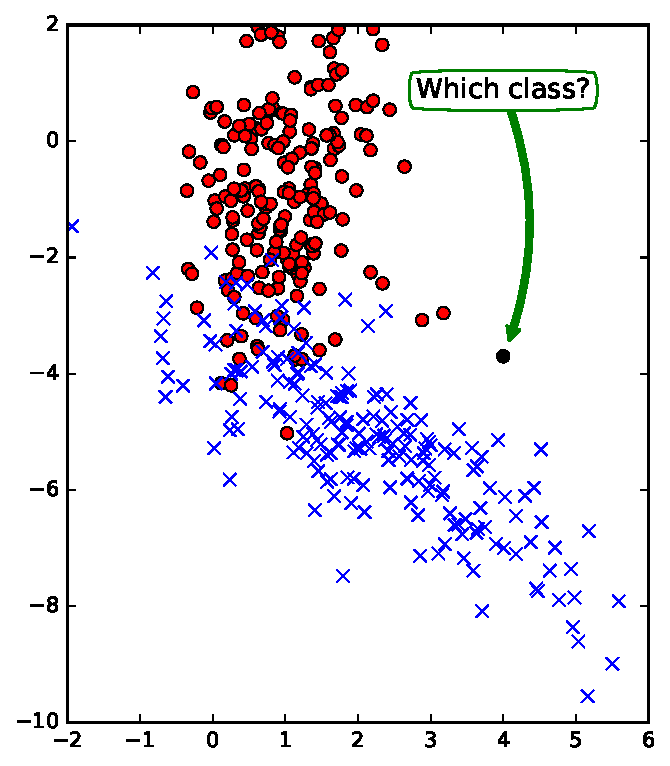
\includegraphics[width=1.2\columnwidth]{twoClassExample.pdf}}
\end{columns}
\end{frame}

\begin{frame}{Regression Example}
\begin{columns}
\column{0.7\textwidth}
\begin{itemize}
\item For example, consider the 1-dimensional data on the right.
\item The data consists of 100 data points, where y coordinate is a function of x.
\item Based on these data, what would be a good prediction of the target value at $x = 1.3$
(the dashed line)?
\item An obvious solution is to fit a curve into the data points.
What kind of forms may the curve have?
\begin{itemize}
\item Straight lines?
\item Continuous curves?
\end{itemize}
\end{itemize}
\column{0.35\textwidth}
\centerline{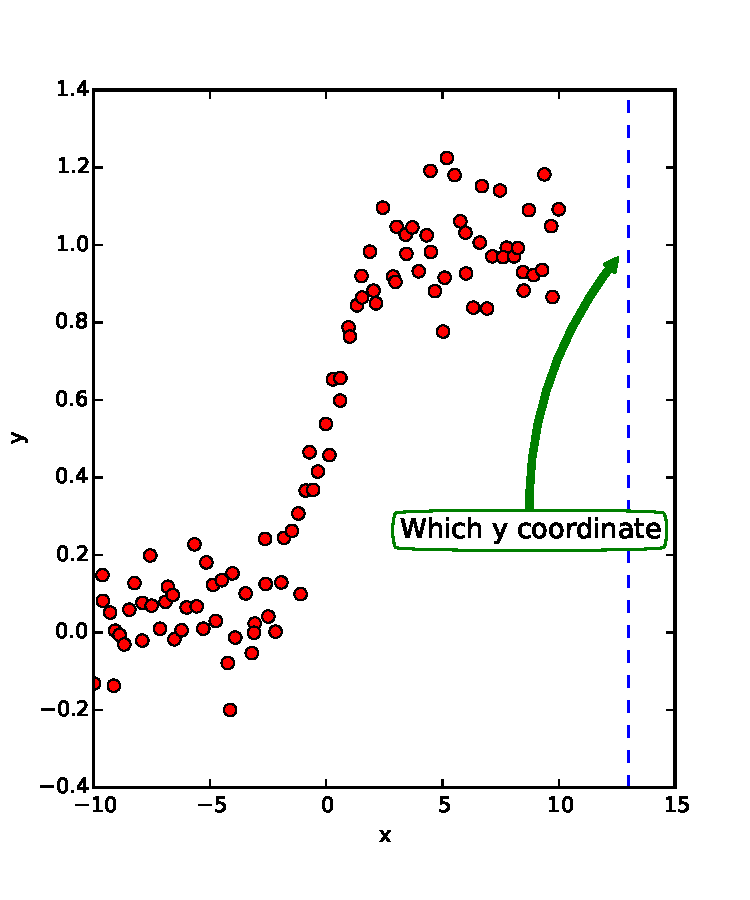
\includegraphics[width=1.2\columnwidth]{regressionExample.pdf}}
\end{columns}
\end{frame}


\begin{frame}{Different Classifiers}
\begin{itemize}
\item We will study the following
widely used classifiers.
\begin{itemize}
\item Nearest Neighbor classifier
\item Linear classifiers (with linear boundary)
\item The support vector machine (with nonlinear boundary)
\item Ensemble classifiers: Random Forest
\item Black boxes: Neural networks and deep neural networks
\end{itemize}
\item For the first four, we will refer to the \emph{Scikit-Learn}
module: \url{http://scikit-learn.org/}.
\item The neural network part will be studied with the \emph{Keras} package: \url{http://keras.io/}.
\end{itemize}
\end{frame}


\begin{frame}{Scikit-Learn}
\begin{itemize}
\item Scikit-Learn started as a Google Summer of Code project.
\item The project became a success: There was a clear need for free elegant platform bringing together
widely used methods.
\item Instead of each contributor providing their own package, scikit-learn has a unified
API for each method.
%\item Altogether over 20 k commits from over 500 contributors.
\item For details: Pedregosa, \textit{et al.} ''Scikit-learn: Machine learning in Python,'' \textit{The Journal of Machine Learning Research},2011.
\end{itemize}
\centerline{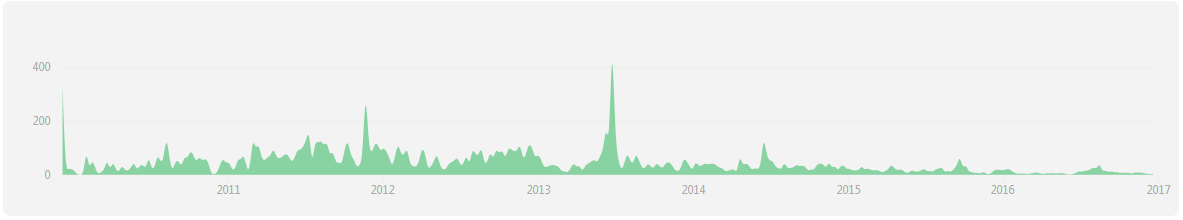
\includegraphics[width=0.8\textwidth]{sklearn-pulse.png}}
\end{frame}

\begin{frame}[fragile,allowframebreaks=0.8]{Scikit-Learn Methods}
Sklearn API is straightforward:
\begin{itemize}
\item \textbf{Initialization:} Each model has its own constructor, \textit{e.g.,}
\verb+model = LogisticRegression(penalty = "l1", C = 0.1)+.
\item \textbf{Training:} Every model implements a \verb+.fit()+ method that
trains the model; \textit{e.g.}, 
\verb+model.fit(X_train, y_train)+
\item \textbf{Prediction:} Every model implements a \verb+.predict()+ method that
predicts the target output for new inputs; \textit{e.g.}, 
\verb+y_hat = model.predict(X_test)+
\item \textbf{Probabilities:} Many models also implement a \verb+.predict_proba()+ method that
predicts the class probabilities for new inputs; \textit{e.g.}, 
\verb+p = model.predict_proba(X_test)+
\end{itemize}
\end{frame}


\begin{frame}[fragile,allowframebreaks=0.8]
 {Sample Scikit-learn Session}
\begin{columns}[onlytextwidth]
\column{0.55\textwidth}
\begin{lstlisting}
# Training code:
from sklearn.linear_model import LogisticRegression

model = LogisticRegression()
model.fit(X, y)
\end{lstlisting}
\begin{lstlisting}
# Testing code:
>>> model.predict([1,2])
array([ 1.])

>>> model.predict([-10,-2])
array([ 0.]

>>> model.predict_proba([[1,2], [-10,-2]])
Out[35]: 
array([[ 0.0044881 ,  0.9955119 ],
       [ 0.56097861,  0.43902139]])
			
# [1,2] is class 1 with 99.5 % confidence.
# [-10,-2] is class 0 with 56.1 % confidence.
\end{lstlisting}
\column{0.5\textwidth}
\begin{itemize}
\item In the example code, \verb+X+ consists of 400 two-dimensional samples from two classes.
\end{itemize}
\centerline{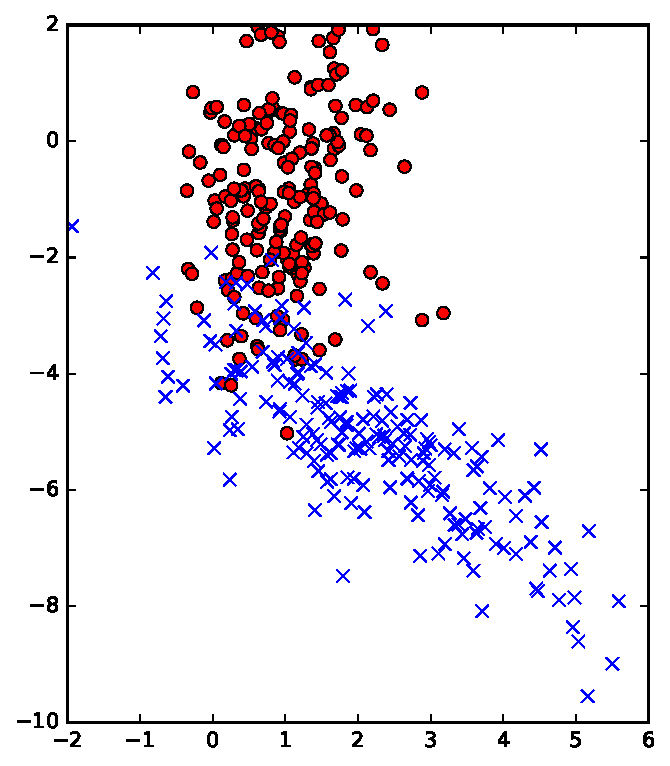
\includegraphics[width=0.7\columnwidth]{twoClassExample_plain.pdf}}
\end{columns}
\end{frame}

\begin{frame}{Nearest Neighbor Classifier}
\begin{columns}
\column{0.7\textwidth}
\begin{itemize}
\item Probably the most natural approach for deciding the class is
simply to see what kind of samples are nearby.
\item This is the idea behind the \textbf{Nearest neighbor} classifier: Just copy
the class label of the most similar training sample to the unknown test sample.
\end{itemize}
\column{0.3\textwidth}
\centerline{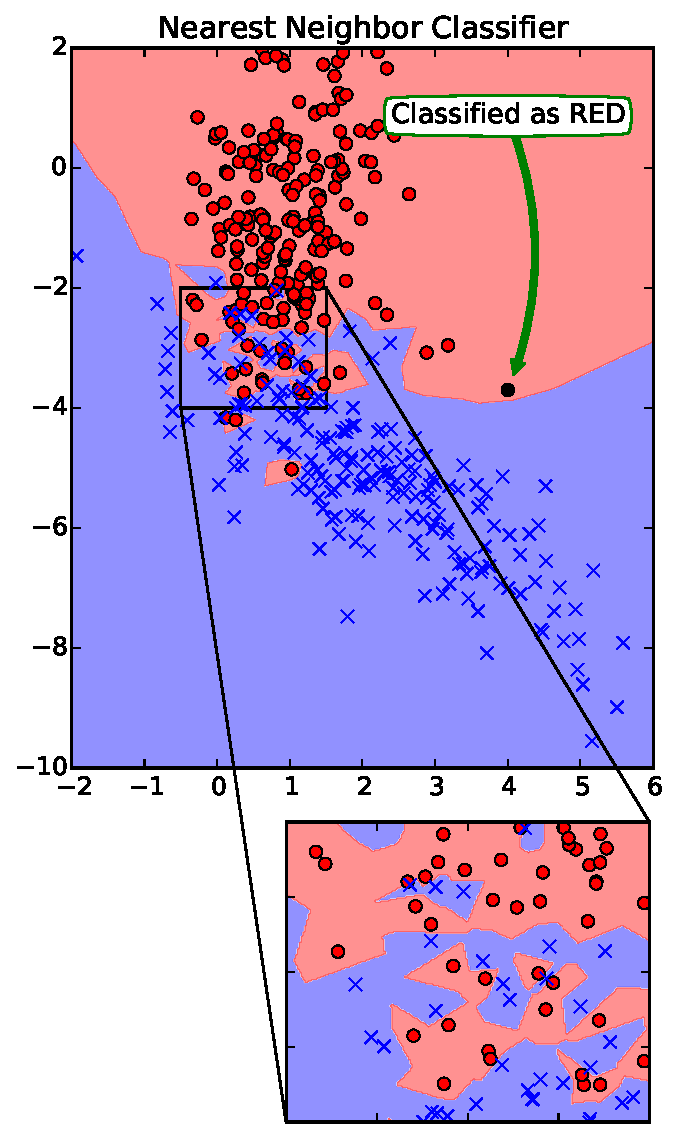
\includegraphics[width=1.0\columnwidth]{1NN.pdf}}
\end{columns}
\end{frame}

\begin{frame}{K-Nearest Neighbor Classifier}
\begin{columns}
\column{0.7\textwidth}
\begin{itemize}
\item The problem with Nearest Neighbor is its fragility to changes in the training data.
\item The classification boundary may change a lot by moving only one training sample.
\item The robustness can be increased by taking a majority vote of more nearby samples.
\item The  \textbf{K-Nearest neighbor} classifier selects the most frequent class label among
the $K$ nearest training samples.
\end{itemize}
\column{0.3\textwidth}
\centerline{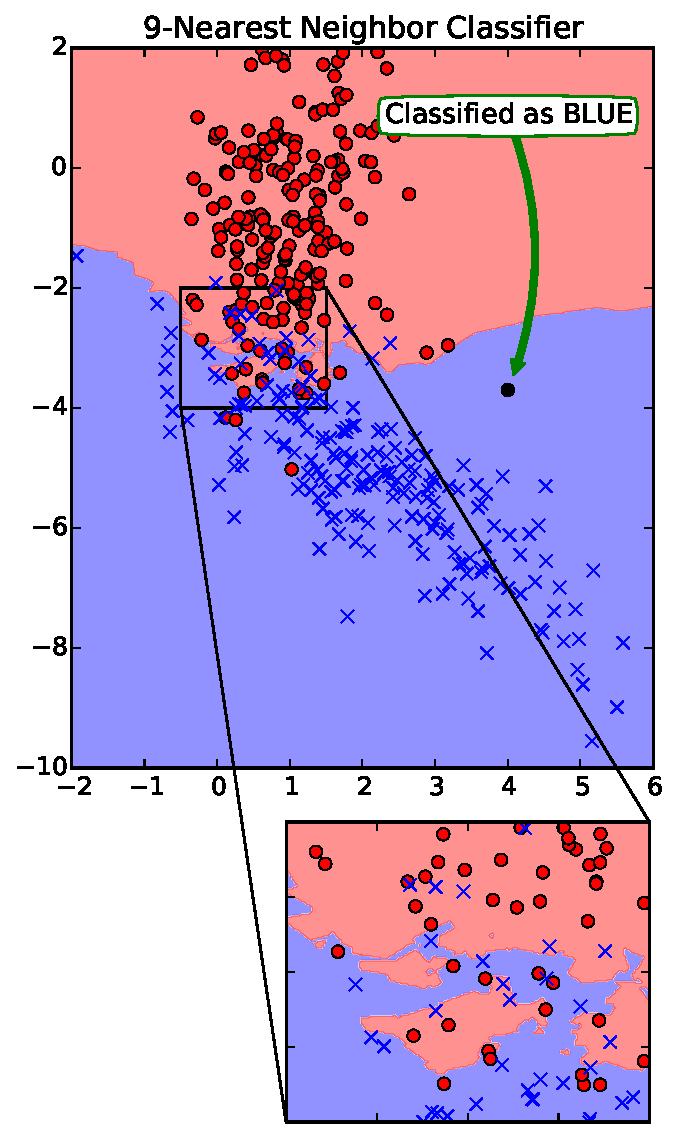
\includegraphics[width=\columnwidth]{9NN.pdf}}
\end{columns}
\end{frame}

\begin{frame}[fragile,allowframebreaks=0.8]
 {Nearest Neighbor in Scikit-learn}
\begin{columns}[onlytextwidth]
\column{0.52\textwidth}
\begin{lstlisting}
# Training code:
from sklearn.neighbors import KNeighborsClassifier

model = KNeighborsClassifier(n_neighbors = 5, metric = "euclidean")
model.fit(X, y)
\end{lstlisting}
\begin{lstlisting}
# Testing code:
>>> model.predict([-10,-2])
array([ 0.])

>>> model.predict([1,2])
array([ 1.])

>>> model.predict_proba([0,-3])
array([[ 0.6,  0.4]])

# Ask what are the 5 nearest neighbors.
# Returns the distances and indices (rows) in X
>>> distances, indices = model.kneighbors([0,-3])
[0.144,  0.254,  0.362,  0.414,  0.422]
[379,  11, 215, 370, 198]

# What are the classes for these five:
>>> y[indices]
array([[ 0.,  1.,  0.,  0.,  1.]])
\end{lstlisting}
\column{0.48\textwidth}
\begin{itemize}
\item Parameters of constructor include:
\begin{itemize}
\item \verb+n_neighbors+: Number of neighbors $K$
\item \verb+metric+: How distance is calculated
\item \verb+algorithm+: Which algorithm finds the nearest samples;
\textit{e.g.,} methods like \textit{K-D Tree} or \textit{brute force}
\end{itemize}
\item Probability prediction counts how many of the nearest $K$ samples belong
to each group.
\item Thus, the probabilities are very quantized and often either $0$ or $1$.
\end{itemize}
\end{columns}
\end{frame}

\begin{frame}{Benefits of Nearest Neighbor}
%\begin{columns}
%\column{0.7\textwidth}
\begin{itemize}
\item Training time is minimal: Either just store the data as is; or reorganize it into a tree structure for efficient search.
\item Accuracy is often relatively good. 
\item Allows complicated definitions of distance, \textit{e.g.},
\begin{itemize}
\item Find the 5 nearest samples holding attributes A and B but not C.
\end{itemize}
\item New data can be added/deleted without retraining.
\end{itemize}
%\column{0.35\textwidth}
%\centerline{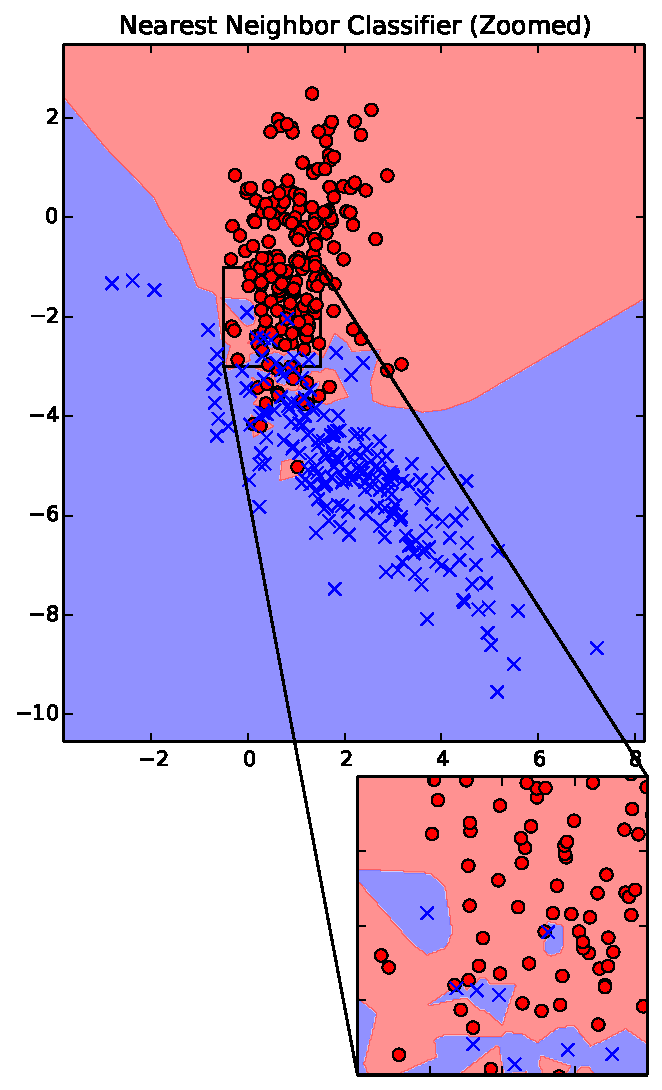
\includegraphics[width=1.2\columnwidth]{1NN_zoom.pdf}}
%\end{columns}
\end{frame}


\begin{frame}{Problems with the Nearest Neighbor}
%\begin{columns}
%\column{0.7\textwidth}
\begin{itemize}
\item Nearest neighbor is prone to overlearning: Especially the 1-NN forms local
regions around every isolated data point. 
\item It is highly unlikely that these represent the general trend of the whole population.
\item Moreover, the training step extremely fast while the classification step becomes
extremely slow (consider training data with billion high-dimensional samples).
\item Therefore, more compact representations are preferred: Training time is
usually not critical while execution time is.
\end{itemize}
%\column{0.35\textwidth}
%\centerline{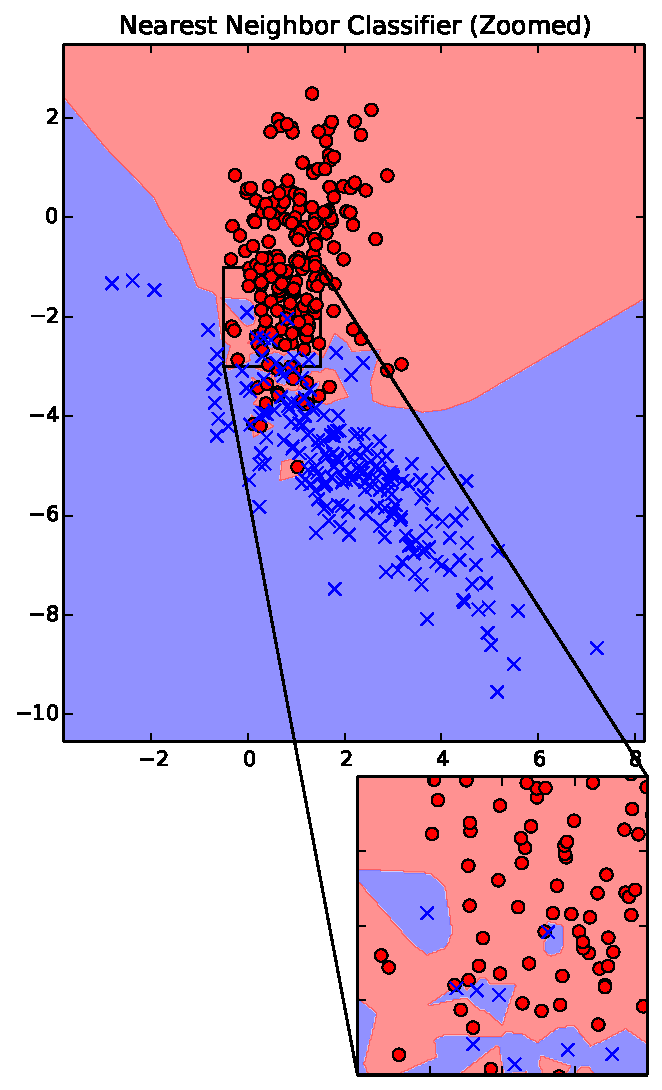
\includegraphics[width=1.2\columnwidth]{1NN_zoom.pdf}}
%\end{columns}
\end{frame}

\begin{frame}{Linear Classifiers}
\begin{columns}
\column{0.7\textwidth}
\begin{itemize}
\item A linear classifier learns a linear decision boundary between classes.
\item In mathematical terms, the classification rule can be written as
\[
F(\x) = \begin{cases}
\text{Class 1,} & \text{if } \w^T\x < b\\
\text{Class 2,} & \text{if } \w^T\x \geq b
\end{cases}
\]
where the weights $\w$ are learned from the data.
\item The expression $\w^T\x = \sum_k w_kx_k$ essentially transforms the 
multi\-dimensional data $\x$ to a real number, which is then compared to a threshold $b$.
\end{itemize}
\column{0.3\textwidth}
\centerline{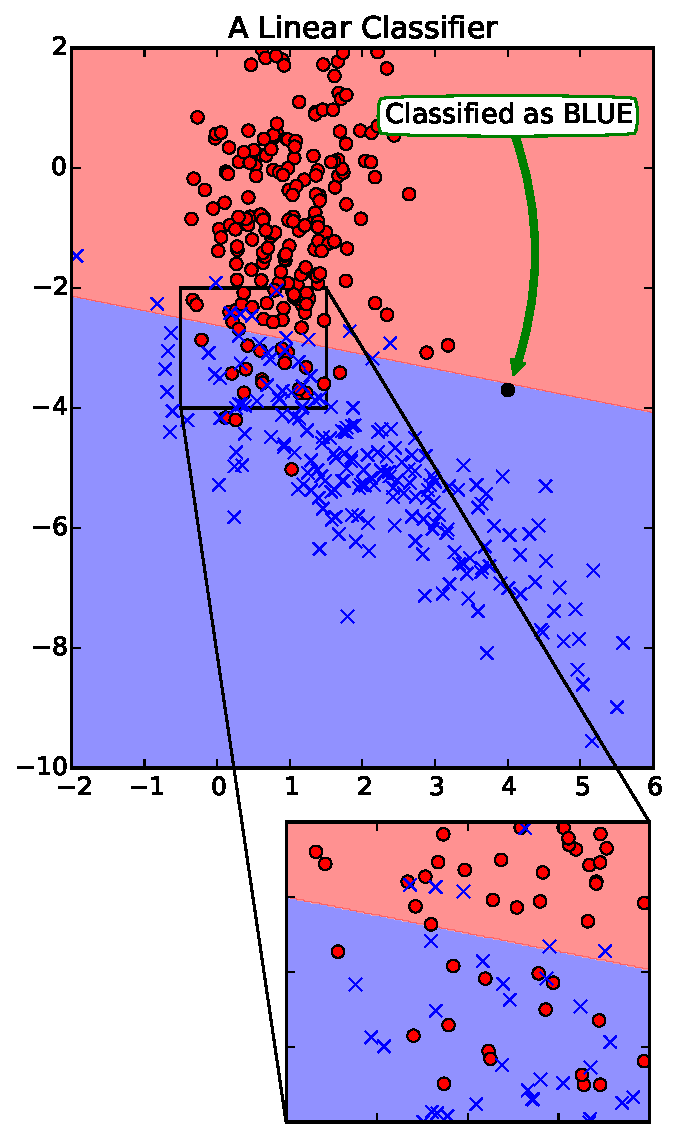
\includegraphics[width=\columnwidth]{Linear.pdf}}
\end{columns}
\end{frame}

\begin{frame}{Flavors of Linear Classifiers}

There exists many algorithms for learning the weights $\w$, including:

{\footnotesize\em
\begin{columns}
\hspace*{0.3cm}
\column{0.33\textwidth}
\begin{itemize}
\item Linear Discriminant Analysis (LDA)
\end{itemize}
\centerline{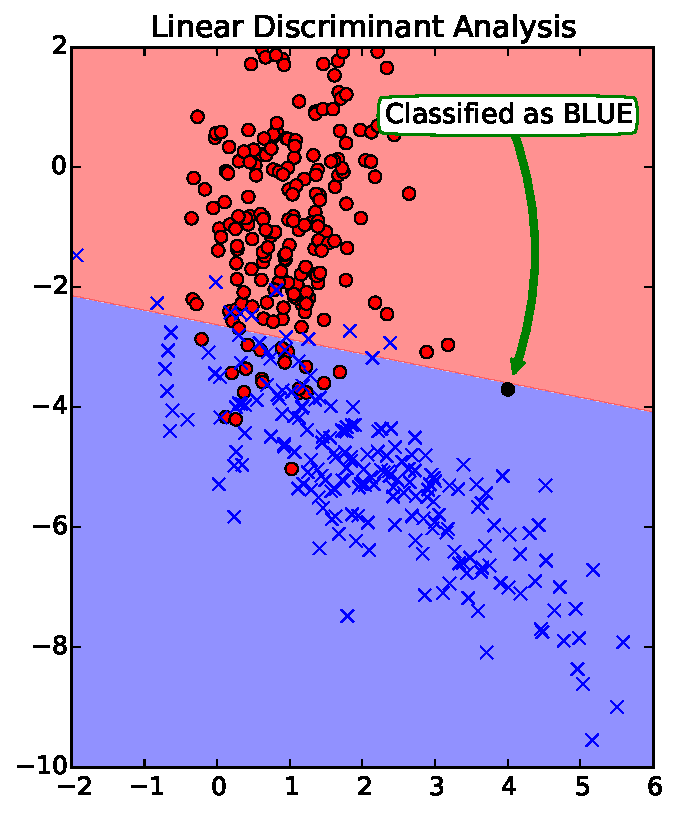
\includegraphics[width=\columnwidth]{LDA.pdf}}
\column{0.33\textwidth}
\begin{itemize}
\item Support Vector Machine (SVM)
\end{itemize}
\centerline{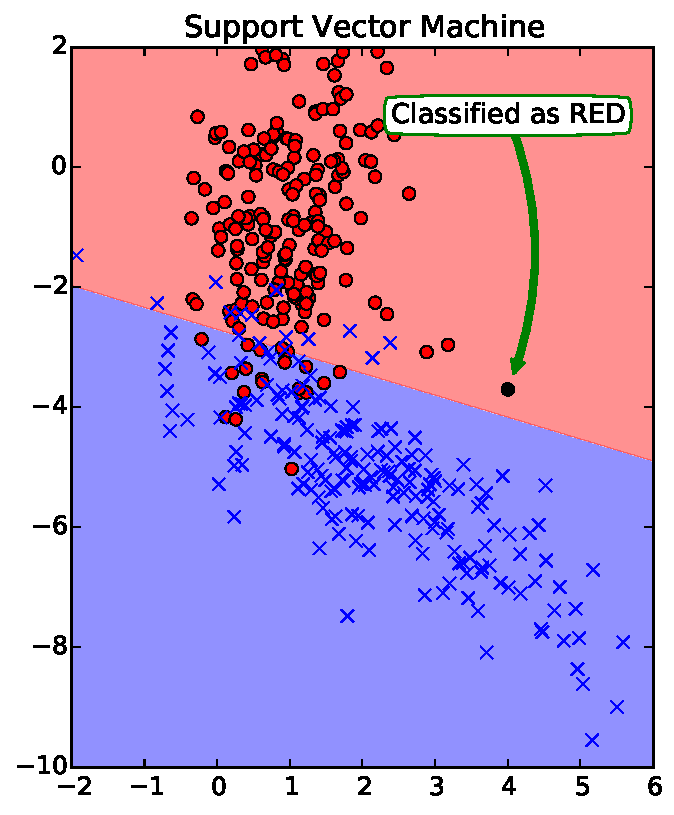
\includegraphics[width=\columnwidth]{SVM.pdf}}
\column{0.33\textwidth}
\begin{itemize}
\item Logistic Regression (LR)
\end{itemize}
\centerline{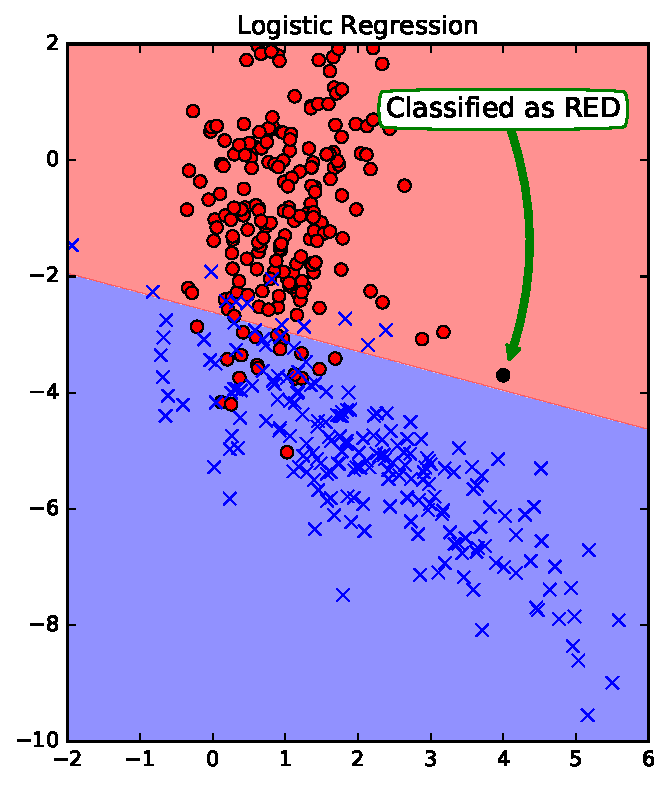
\includegraphics[width=\columnwidth]{LR.pdf}}
\end{columns}
}
\end{frame}

\begin{frame}{Flavors of Linear Classifiers}
%\begin{columns}
%\column{0.7\textwidth}
\begin{itemize}
\item The LDA:
\begin{itemize}
\item The oldest of the three: Fisher, 1935.
\item "Find the projection that maximizes class separation", \emph{i.e.}, pull the 
classes as far from each other as possible.
\item Closed form solution, fast to train.
\end{itemize}

\item The SVM:
\begin{itemize}
\item Vapnik and Chervonenkis, 1963.
\item "Maximize the margin between classes". 
\item Slowest of the three\footnote{Slowest in \emph{training}; testing time is the same for all}, performs well with sparse high-dimensional data.
\end{itemize}

\item Logistic Regression (\emph{a.k.a.} \emph{Generalized Linear Model}):
\begin{itemize}
\item History traces back to 1700's, but proper formulation and efficient training algorithm 
by Nelder and Wedderburn in 1972.
\item Statistical algorithm: "Maximize the likelihood of the data". 
\item Outputs also class probability. Has been extended to automatic feature selection.
\end{itemize}

\end{itemize}
%\column{0.35\textwidth}
%\centerline{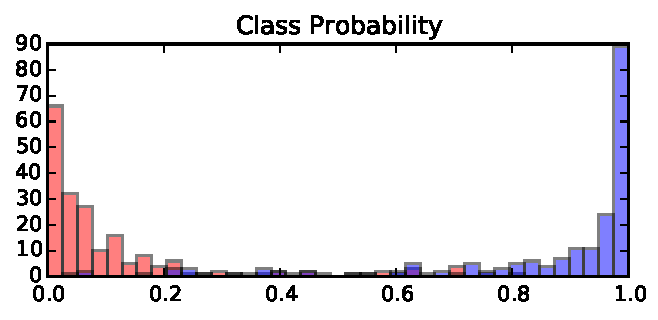
\includegraphics[width=1.2\columnwidth]{LR_prob.pdf}}
%\end{columns}
\end{frame}


\begin{frame}{Linear Discriminant Analysis}
\begin{columns}
\column{0.35\textwidth}
\begin{itemize}
\item The LDA maps high dimensional data into a single scalar simultaneously pulling individual
classes apart.
\item Thus, the task is essentially finding a good linear projection $\R^N \mapsto \R$.
\end{itemize}
\column{0.65\textwidth}
\begin{center}
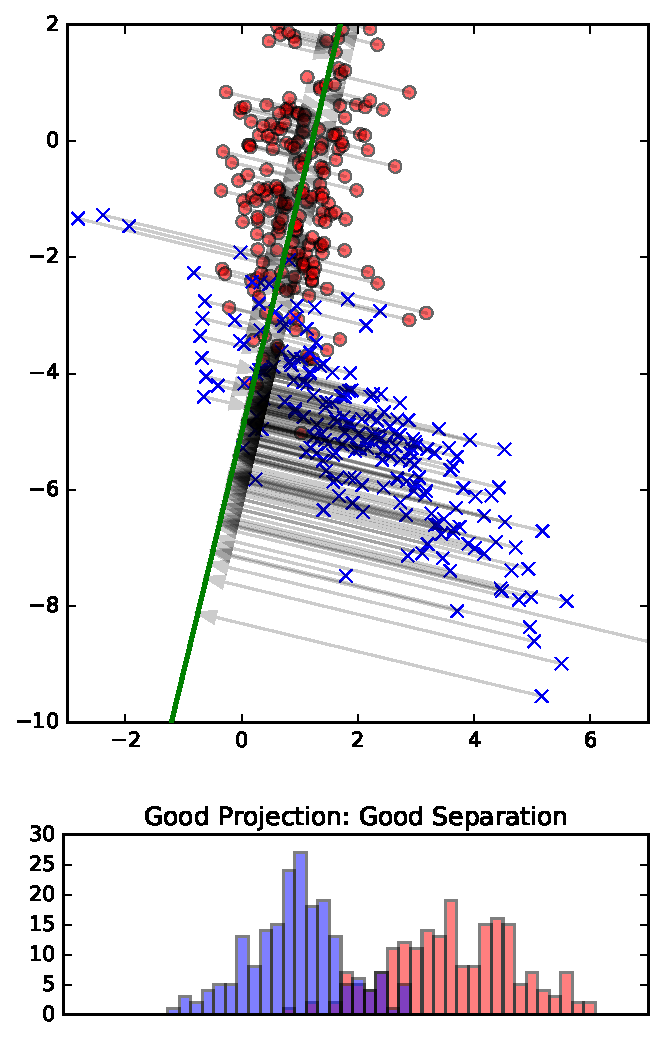
\includegraphics[width=0.47\textwidth]{LDA_proj1.pdf}
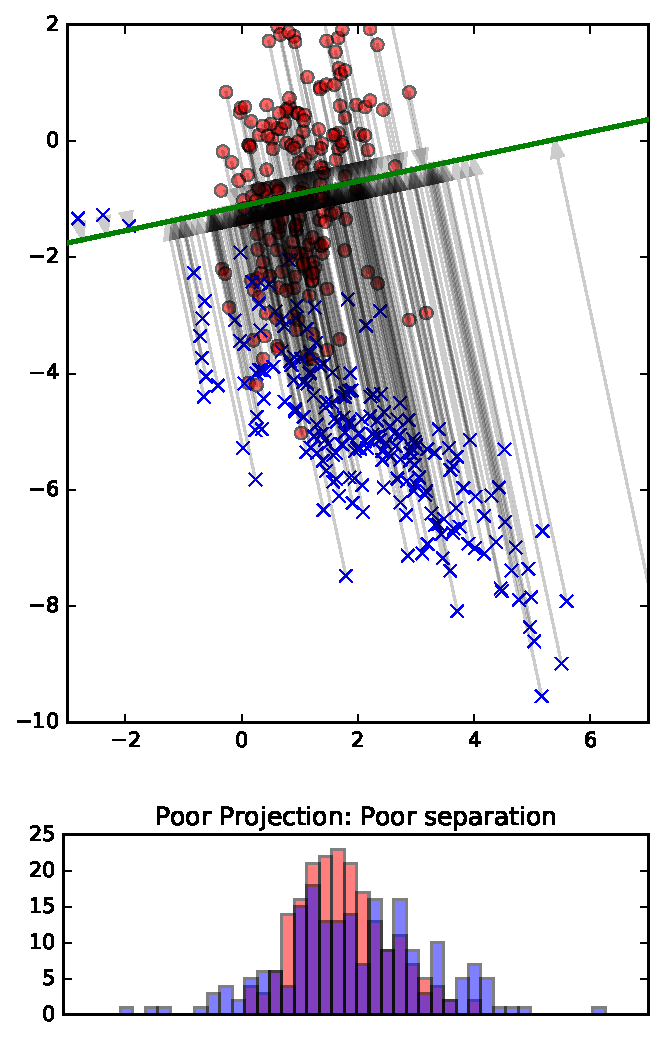
\includegraphics[width=0.47\textwidth]{LDA_proj2.pdf}
\end{center}
\end{columns}
\end{frame}

\begin{frame}{Linear Discriminant Analysis}
\begin{itemize}
\item A good measure of class separation could be,\textit{ e.g.}, the distance between their projected means.
\item However, this quantity depends on the scale, and increases simply by multiplying by a large number.
\item Thus, we want to pull class means apart while keeping the variance of each class small.
\item As a result, we look into the following separability score:
\begin{align*}
J(\w) &= \frac{\text{Distance of Class Means}}{\text{Variance of Classes}}\\
&= \frac{(\w^T\mub_1 - \w^T\mub_0)^2}{\w^T\Sigb_1\w + \w^T\Sigb_0\w},
\end{align*}
where $\mub_1$ and $\mub_0$ are the class means and $\Sigb_1$ and $\Sigb_0$ covariance matrices of the
two classes.
\end{itemize}
\end{frame}

\begin{frame}{Maximization of $J(\w)$}
\begin{itemize}
\item The Fisher separation score can be maximized analytically.
\item First simplify $J(\w)$ a bit:
\[
J(\w) = \frac{(\w^T\mub_1 - \w^T\mub_0)^2}{\w^T\Sigb_1\w + \w^T\Sigb_0\w} = \frac{\w^T\SB_B\w}{\w^T\SB_W\w}
\]
with $\SB_B = (\mub_1 - \mub_0)(\mub_1 - \mub_0)^T$ and $\SB_W = \Sigb_1 + \Sigb_0$.
\item This form is known as \textit{Generalized Rayleigh Quotient}, which appears in many contexts.
\item Using Lagrange multipliers, one can show that the maximum must satisfy
\[
\SB_B\w = \lambda \SB_W\w
\]
with $\lambda \in \R$ a constant. 
\end{itemize}
\end{frame}

\begin{frame}{Maximization of $J(\w)$}
\begin{itemize}
\item The above condition is a \textit{generalized eigenvalue problem}.
\item In other words, there are many solutions: one for each eigenvalue.
\item Thus, it is straightforward to conclude that the quantity
\[
J(\w) = \frac{\w^T\SB_B\w}{\w^T\SB_W\w}
\]
is maximized when
\[
\SB_B\w = \lambda \SB_W\w
\]
or equivalently
\[
\w^T\SB_B\w = \lambda \w^T\SB_W\w
\]
\item Finally, the ratio $\w^T\SB_B\w  / \w^T\SB_W\w$ is maximized by choosing
$\lambda$ as the largest eigenvalue (and $\w$ as the corresponding eigenvector).
\end{itemize}
\end{frame}

\begin{frame}[fragile,allowframebreaks=0.8]
 {Solution 1 using Eigenvalues}
\begin{columns}[onlytextwidth]
\column{0.5\textwidth}
\begin{lstlisting}
# Training code:
import numpy as np
from scipy.linalg import eig

# X0 and X1 contain data of the 2 classes
m0 = np.mean(X0.T, axis = 0)
m1 = np.mean(X1.T, axis = 0)
C0 = np.cov(X0.T - np.tile(m0, (X0.shape[1], 1)), rowvar = False)
C1 = np.cov(X1.T - np.tile(m1, (X1.shape[1], 1)), rowvar = False)

SB = np.multiply.outer(m1 - m0, m1 - m0)
SW = C0 + C1

D, V = eig(SB, SW)
w = V[:, -1]

T = np.mean([np.dot(m1, w), np.dot(m2, w)])
\end{lstlisting}
\begin{lstlisting}
# Testing code:
>>> w
array([ 0.23535937,  0.97190842])

>>> np.dot(w, [0,-2]) - T
0.606
# Positive -> in class "red circles"

>>> np.dot(w, [0,-3]) - T
-0.3657
# Negative -> in class "blue crosses"
\end{lstlisting}
\column{0.5\textwidth}
\begin{itemize}
\item We need to solve the generalized eigenvalue problem
$\SB_B\w = \lambda \SB_W\w$.
\item \verb+scipy+ has a solver for that.
\item \verb+scipy.linalg.eig+ returns
\begin{itemize}
\item Array of eigenvalues \verb+D+ in increasing order.
\item Matrix of eigenvectors \verb+V+ (in columns).
\end{itemize}
\item Thus, we want the rightmost (''$-1^{\text{th}}$'') column \verb+V[:, -1]+ (corresponding to largest eigenvalue).
\item The decision is done by comparing the projected vector to threshold \verb+T+; the center of projected class means.
\end{itemize}
\end{columns}
\end{frame}

\begin{frame}{LDA Projection with Threshold}
\centerline{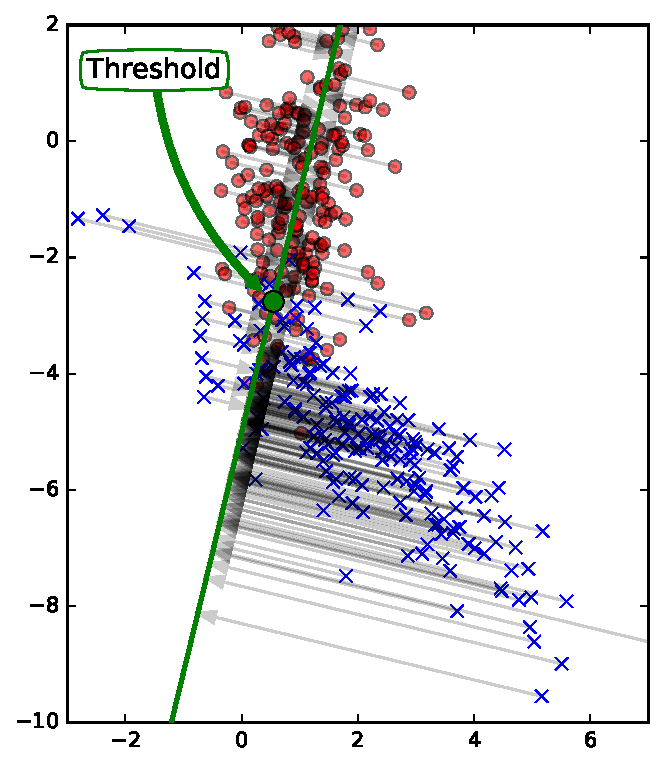
\includegraphics[width=0.4\columnwidth]{LDA_proj1_threshold.pdf}}
\end{frame}

\begin{frame}[fragile,allowframebreaks=0.8]
 {Solution 2 without Eigenvalues}
\begin{itemize}
\item It turns out that solving the generalized eigenvalue problem $\SB_B\w = \lambda\SB_W\w$ is not necessary. 
\item The maximum of $J(\w)$ has to satisfy $\SB_B\w = \lambda\SB_W\w$, or equivalently,
$\SB_W^{-1}\SB_B\w = \lambda\w$.
\item Insert the definition of $\SB_B$ to get:
\[
\SB_W^{-1}(\mub_1 - \mub_0)\underbrace{(\mub_1 - \mub_0)^T\w}_{\text{scalar } C} = \lambda\w
\]
or,
\[
\SB_W^{-1}(\mub_1 - \mub_0) \frac{C}{\lambda} = \w
\]
\item Thus, the maximum of $J(\w)$ has to satisfy this condition as well (regardless of $\lambda$).
\item We are  looking for a direction
vector $\w$, so the multiplier $C / \lambda$ is not relevant either ($\frac{c}{\lambda}\w$ has the same direction as $\w$).
\item Thus, $\w$ is given by 
\[
\w = \SB_W^{-1}(\mub_1 - \mub_0) = (\Sigb_0 + \Sigb_1)^{-1}(\mub_1 - \mub_0).
\]
\end{itemize}
\end{frame}

\begin{frame}[fragile,allowframebreaks=0.8]
 {Solution 2 without Eigenvalues}
\begin{columns}[onlytextwidth]
\column{0.5\textwidth}
\begin{lstlisting}
# Training code:
import numpy as np
from scipy.linalg import eig

# X0 and X1 contain data of the 2 classes
m0 = np.mean(X0.T, axis = 0)
m1 = np.mean(X1.T, axis = 0)

C0 = np.cov(X0.T - np.tile(m0, (X0.shape[1], 1)), rowvar = False)
C1 = np.cov(X1.T - np.tile(m1, (X1.shape[1], 1)), rowvar = False)

w = np.dot(np.linalg.inv(C0 + C1), (m1 - m0))

T = np.mean([np.dot(m1, w), np.dot(m2, w)])
\end{lstlisting}
\begin{lstlisting}
# Testing code:
>>> w
array([ 0.25237576,  1.04217702])

>>> np.dot(w, [0,-2]) - T
0.65004
# Positive -> in class "red circles"

>>> np.dot(w, [0,-3]) - T
-0.3921
# Negative -> in class "blue crosses"
\end{lstlisting}
\column{0.5\textwidth}
\begin{itemize}
\item The Python code is very similar to the eigenvalue based solution.
\item Note that the resulting \verb+w+ is not exactly the same: The lengths
are different, but directions are the same.
\end{itemize}
\centerline{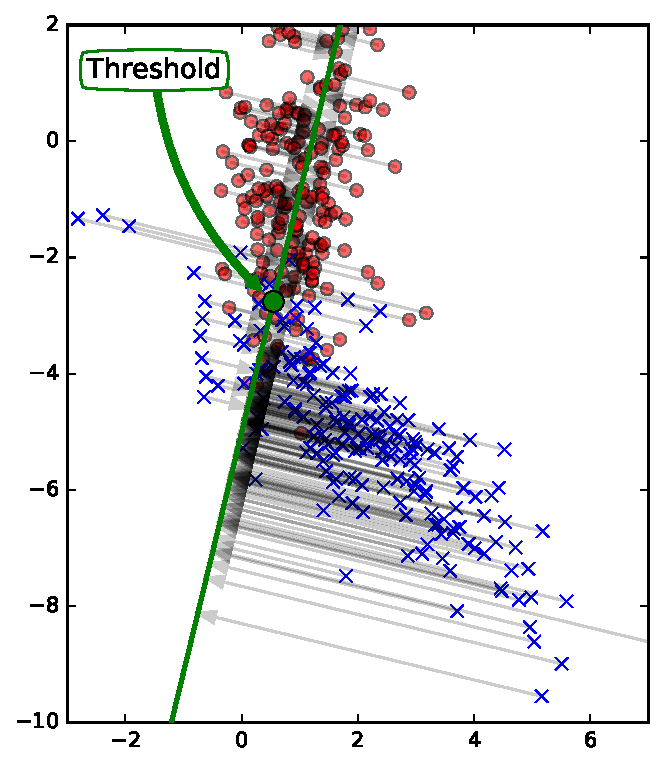
\includegraphics[width=0.6\columnwidth]{LDA_proj1_threshold.pdf}}
\end{columns}
\end{frame}

\begin{frame}[fragile,allowframebreaks=0.8]
 {Solution 3: Scikit-Learn}
\begin{columns}[onlytextwidth]
\column{0.45\textwidth}
\begin{lstlisting}
# Training code:
from sklearn.discriminant_analysis import LinearDiscriminantAnalysis

clf = LinearDiscriminantAnalysis()

# X contains all samples, and y their class
# labels: y = [0,1,1,0,...]
clf.fit(X, y)
\end{lstlisting}
\begin{lstlisting}
# Testing code:
>>> clf.coef_      # This is our w vector
array([[ 0.50475151,  2.08435403]])

>>> clf.intercept_ # This is the threshold
array([ 5.46879769])

>>>  clf.predict([0, -2])
array([ 1.])

>>>  clf.predict([0, -3])
array([ 0.])

>>> clf.predict_proba([0, -3])
array([[ 0.68659846,  0.31340154]])
\end{lstlisting}
\column{0.6\textwidth}
\begin{itemize}
\item Scikit-Learn implements LDA in a straightforward manner.
\item First construct your classifier using \verb+LinearDiscriminantAnalysis()+
\item Then train the model using \verb+fit()+
\item Then predict classes using \verb+predict()+
\item Or class probabilities using \verb+predict_proba()+
\end{itemize}
\end{columns}
\end{frame}

\begin{frame}[fragile,allowframebreaks=0.8]{Multiclass LDA}
\begin{columns}
\column{0.7\textwidth}
\begin{itemize}
\item The LDA can be generalized to handle more than 2 classes.
\item \textit{Multiclass LDA} can be understood in two contexts:
\begin{itemize}
\item As \textit{dimensionality reduction:} We seek for a set of projections,
that lower the dimensionality of the data while retaining its original separability.
\item As \textit{classification:} We seek for a set of discriminant functions that 
give a probability score for each class.
\end{itemize}
\item We are more interested in the latter interpretation. 
\end{itemize}
\column{0.35\textwidth}
\centerline{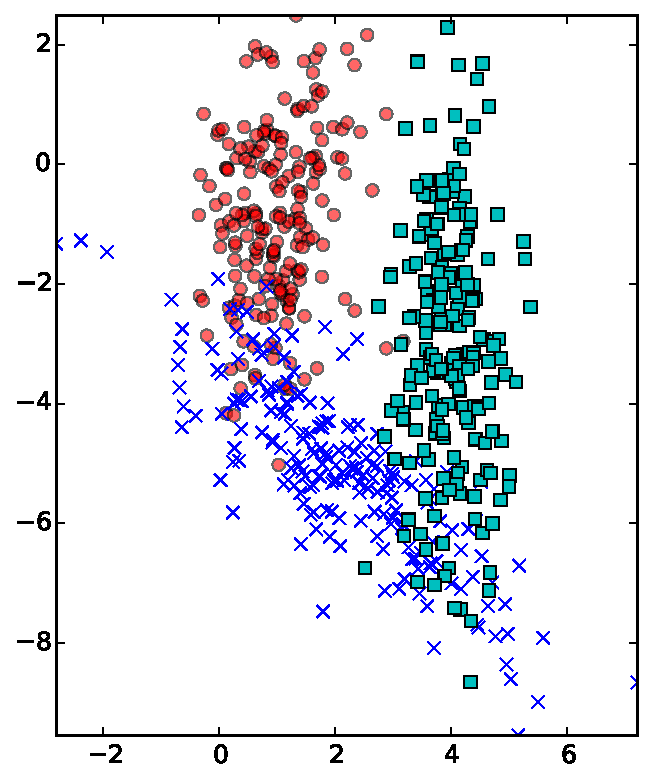
\includegraphics[width=\columnwidth]{3Class_LDA.pdf}}
\end{columns}
\end{frame}

\begin{frame}[fragile,allowframebreaks=0.8]{Multiclass LDA}
\begin{itemize}
\item In this case,
the classifier is defined by a set of linear functions
\begin{align*}
g_1(\x) &= \w_1^T\x + w_1\\
&\vdots \\
g_K(\x) &= \w_K^T\x + w_K\\
\end{align*}
\item Then the vector $\x$ is assigned class $k = 1,2,\ldots, K$ if
\[
g_k(\x) > g_j(\x)
\]
for all $j\ne k$.
\end{itemize}
\end{frame}

\begin{frame}[fragile,allowframebreaks=0.8]
 {Multiclass LDA}
\begin{columns}[onlytextwidth]
\column{0.5\textwidth}
\begin{lstlisting}
# Training code:
import numpy as np
from sklearn.discriminant_analysis import LinearDiscriminantAnalysis

clf = LinearDiscriminantAnalysis()

# X contains all samples, and y their class
# labels: y = [1,3,1,2,...]
clf.fit(X, y)
\end{lstlisting}
\begin{lstlisting}
# Testing code:

# Show the three discriminants (rows):
>>> clf.coef_
array([[-1.00629245,  0.51513354], 
       [-0.74957209, -0.8613368 ], 
       [ 1.75586454,  0.34620326]])

# Compute discriminants for [0,-2]
>>> scores = np.dot(clf.coef_, [0,-2]) + clf.intercept_
array([ 0.56090889, -1.20225066, -6.31434368])
# First class (red) has largest score

# Predict class more easily using predict()
>>> clf.predict([[0, -2], [0, -4]])
array([ 1.,  2.])
\end{lstlisting}
\column{0.5\textwidth}
\begin{itemize}
\item \verb+LinearDiscriminantAnalysis()+ model applies to multiclass case as well.
\item The \verb+fit()+ method finds the three discriminants also shown in the plot below.
\end{itemize}
\centerline{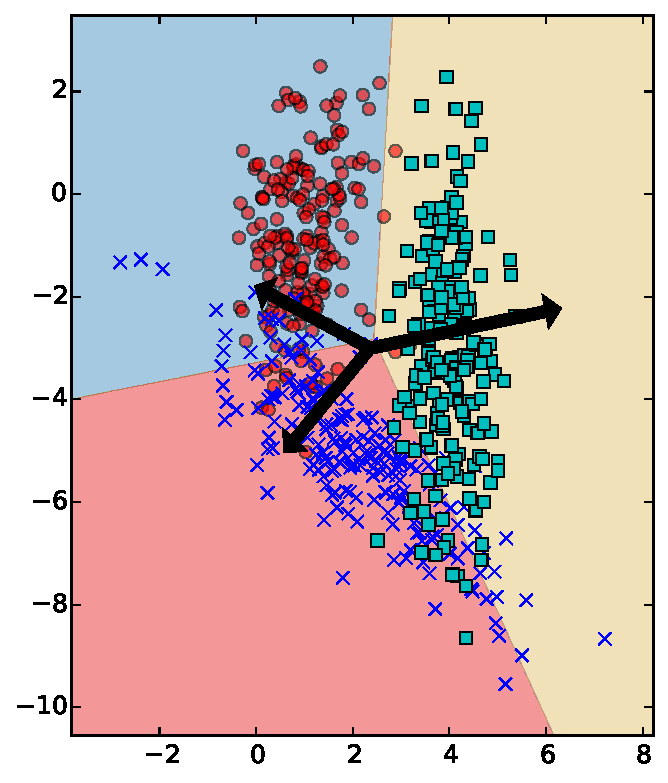
\includegraphics[width=0.55\columnwidth]{3Class_LDA_classes.pdf}}
\end{columns}
\end{frame}

\begin{frame}[fragile,allowframebreaks=0.8]
 {The Support Vector Machine}
\begin{columns}[onlytextwidth]
\column{0.75\textwidth}
\begin{itemize}
\item The Support Vector Machine (SVM) is characterized by its \textit{maximum margin property.}
\item In other words, it attempts to maximize the margin between classes.
\item In the attached example, the binary data is perfectly 
separable, and the SVM sets the boundary in the middle of the two classes.
\item Thus, the boundary location is defined by three samples only; called \textit{support vectors}.
\end{itemize}
\column{0.25\textwidth}
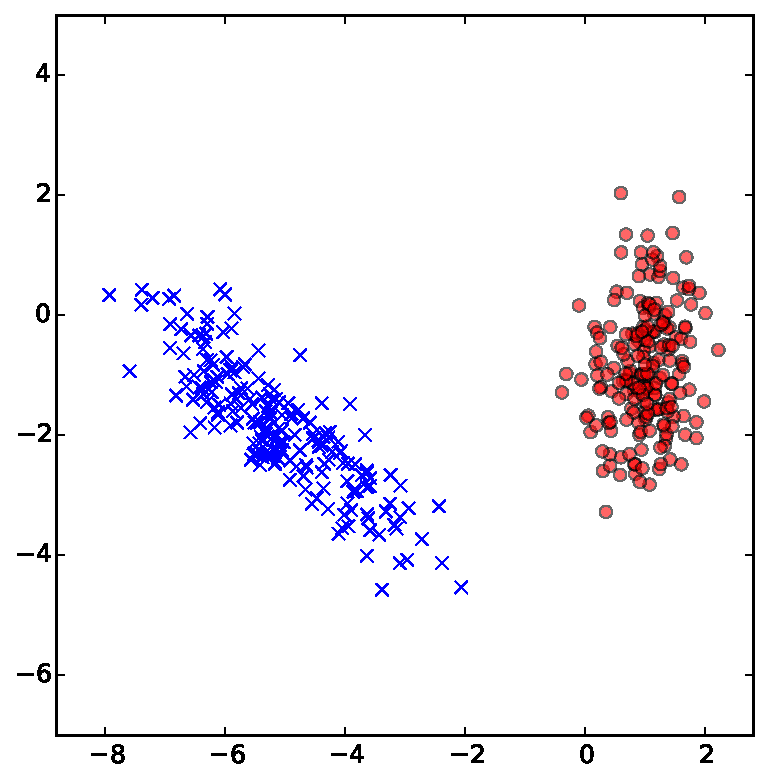
\includegraphics[width=\columnwidth]{SVM_data.pdf}\\
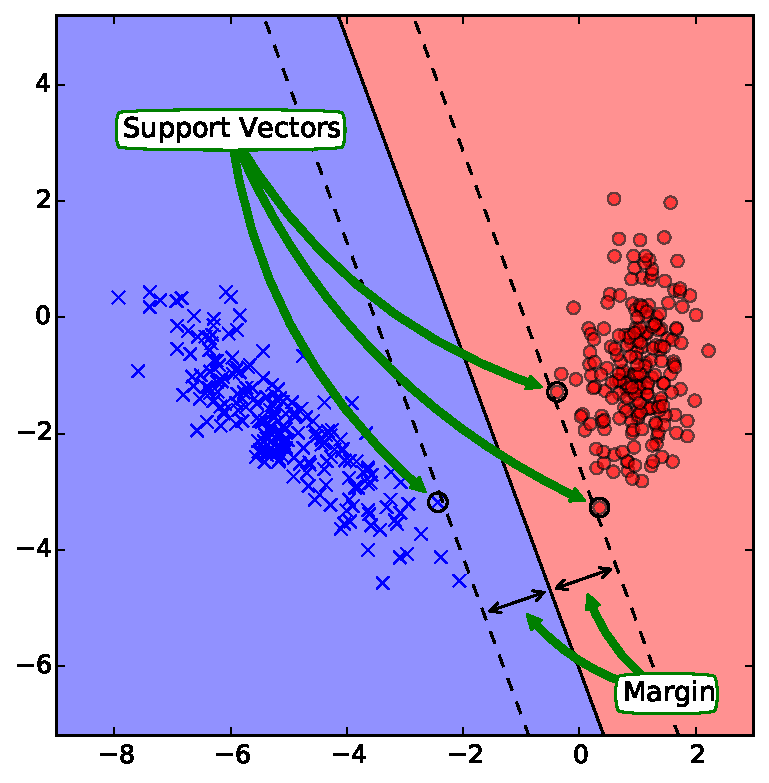
\includegraphics[width=\columnwidth]{SVM_boundary.pdf}
\end{columns}
\end{frame}

\begin{frame}[fragile,allowframebreaks=0.8]
 {The Support Vector Machine}
\begin{columns}[onlytextwidth]
\column{0.75\textwidth}
\begin{itemize}
\item Maximizing the margin $M$ for the SVM can be characterized as an optimization problem
\begin{gather*}
 \mathop{\text{maximize}}_{\w, b, \|\w\| = 1}  \quad M,  \\
 \textit{subject to} \\
 y_i(\x_i^T\w + b) \geq M, \text{ for } i = 1,2,\ldots, N 
\end{gather*}
\item Here, $y_i$ encodes the class as $y_i\in \{-1, 1\}$, so the last condition
can also be written as
\[
\begin{cases}
\x_i^T\w + b 
\geq M, & \text{if } y_i = 1\\
\x_i^T\w + b \leq -M, & \text{if } y_i = -1
\end{cases}
\]
\end{itemize}
\column{0.3\textwidth}
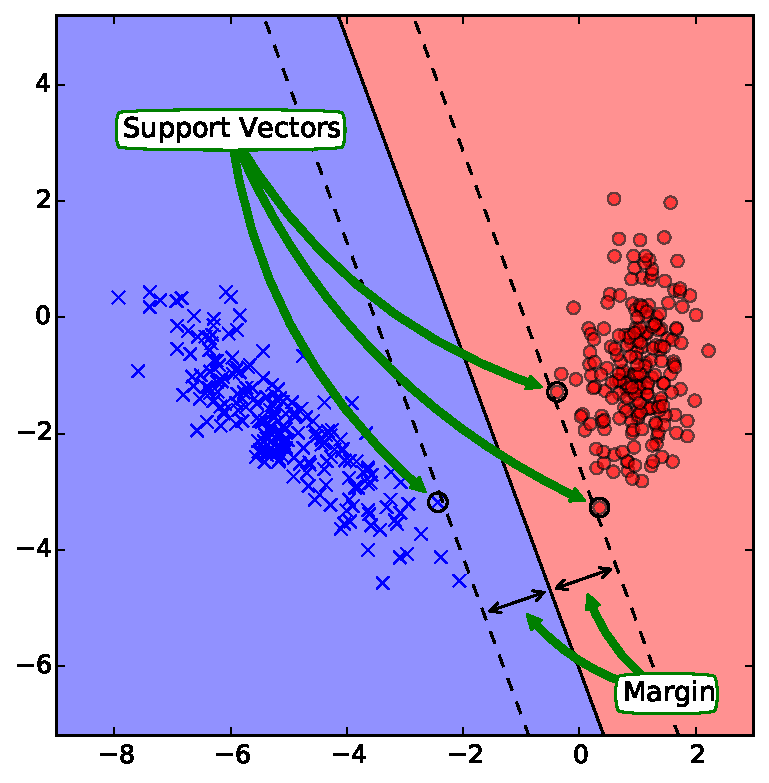
\includegraphics[width=\columnwidth]{SVM_boundary.pdf}
\end{columns}
\end{frame}

\begin{frame}[fragile,allowframebreaks=0.8]
 {The Support Vector Machine}

\begin{itemize}
\item Alternatively, the SVM criterion can be simplified into an equivalent form
\begin{gather*}
 \mathop{\text{minimize}}_{\w, b}  \quad \|\w\|,  \\
 \textit{subject to} \\
 y_i(\x_i^T\w + b) \geq 1, \text{ for } i = 1,2,\ldots, N 
\end{gather*}
\item This is a convex optimization problem with constraints. Efficient
tailored algorithms exist.
\item The implementation of Scikit-learn is based on the widely used
LibSVM library.
\end{itemize}
\end{frame}

\begin{frame}[fragile,allowframebreaks=0.8]
 {The Support Vector Machine}
\begin{columns}[onlytextwidth]
\column{0.7\textwidth}
\begin{itemize}
\item The earlier definition of SVM assumes that the classes are separate (and
there exists a margin between classes).
\item In reality we have to allow some samples to reside on the wrong side of the margin.
\item The solution is to penalize for samples on the wrong side.
\item The resulting function to be minimized is:
\begin{gather*}
\mathop{\text{minimize}}_{\w, b} \sum_{i=1}^{N} [\max(0, 1-y_i(\w^T\x_i + b))] + C\|\w\|^2.
\end{gather*}
\item For each sample on the wrong side, we add a penalty (called \textit{hinge loss}) defined as
\(
\max(0, x)
\)
\item Note, that this increases the number of SV's.
\end{itemize}
\column{0.3\textwidth}
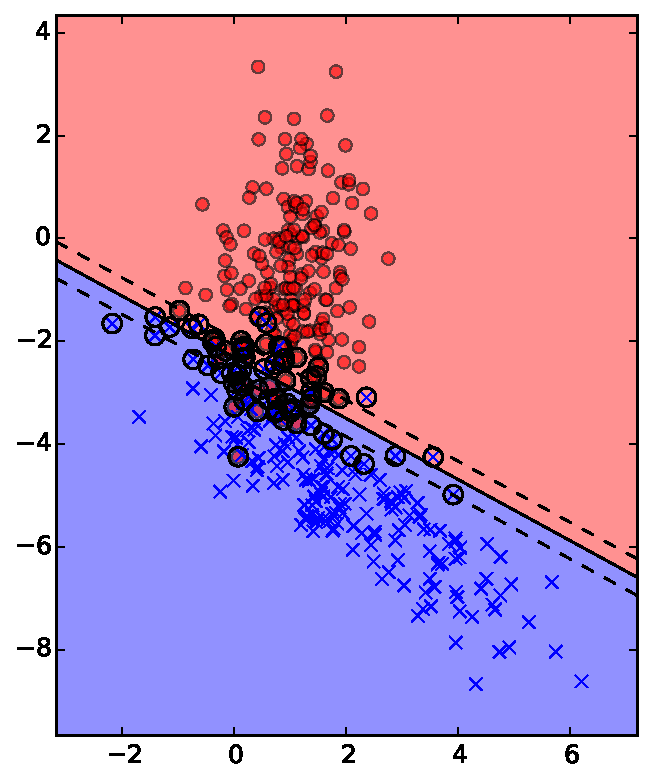
\includegraphics[width=\columnwidth]{SVM_boundary_overlap.pdf}\\
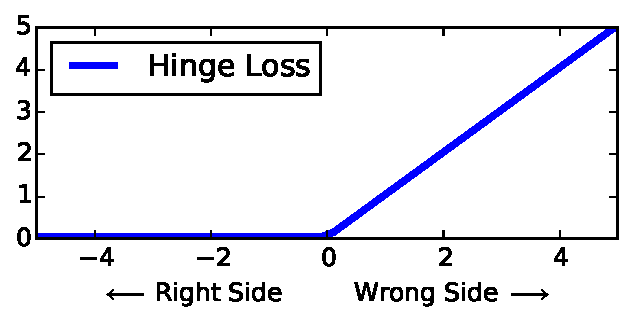
\includegraphics[width=\columnwidth]{hinge_loss.pdf}
\end{columns}
\end{frame}


\begin{frame}[fragile,allowframebreaks=0.8]
{SVM in Scikit-Learn}
\begin{itemize}
\item The parameter $C$ determines the balance between margin width and penalty for being on the wrong side.
\item Left to right: Linear SVM's with decreasing penalty.
\end{itemize}
\begin{center}
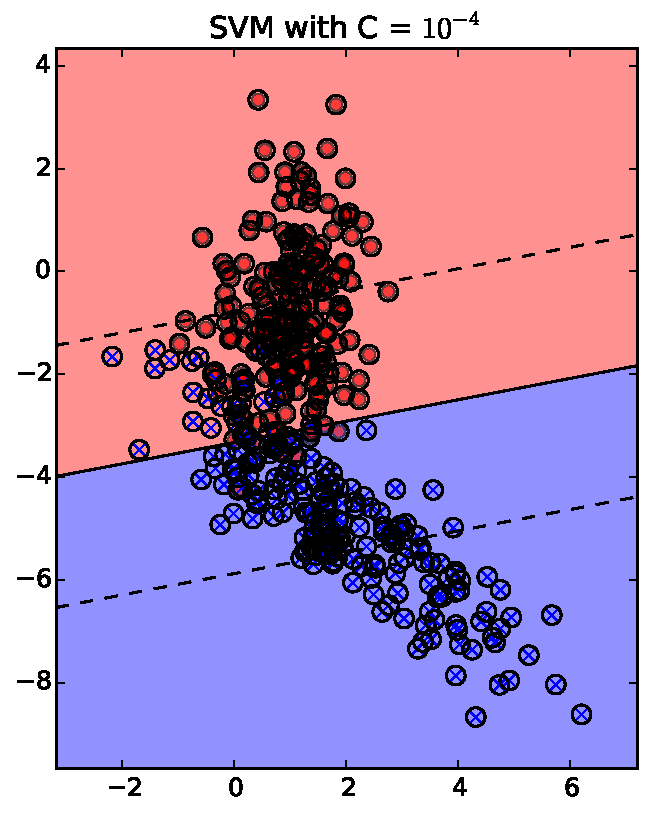
\includegraphics[width=0.2\textwidth]{SVM_C_-4.pdf}
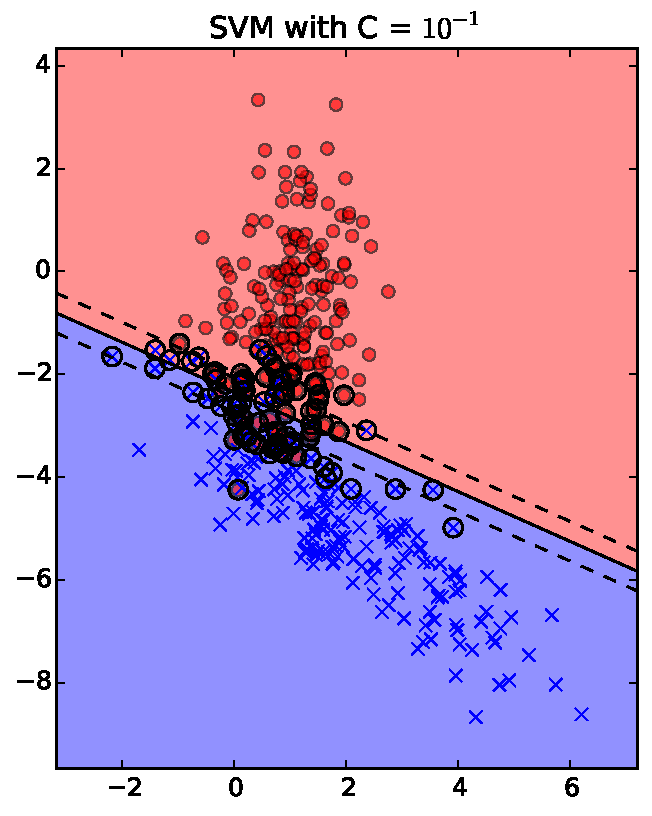
\includegraphics[width=0.2\textwidth]{SVM_C_-1.pdf}
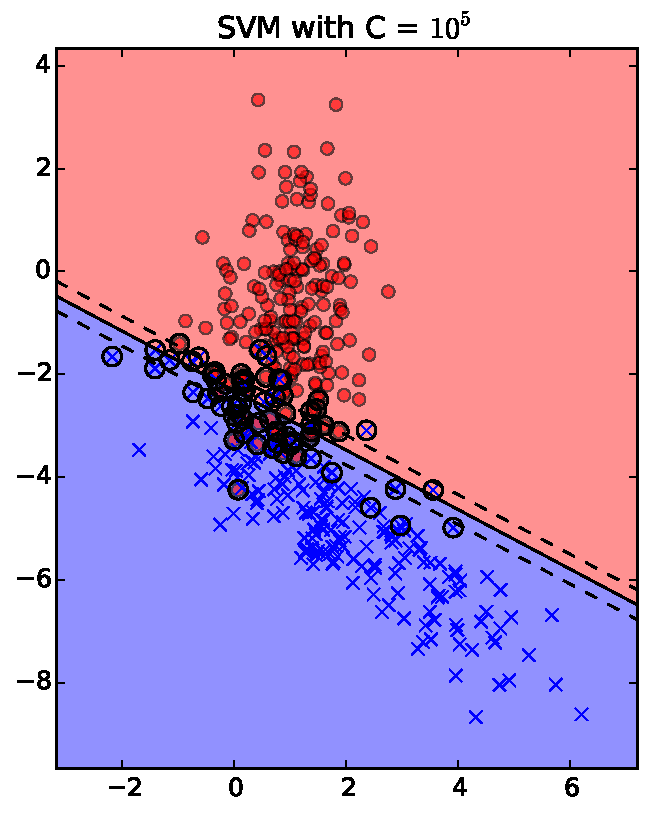
\includegraphics[width=0.2\textwidth]{SVM_C_5.pdf}
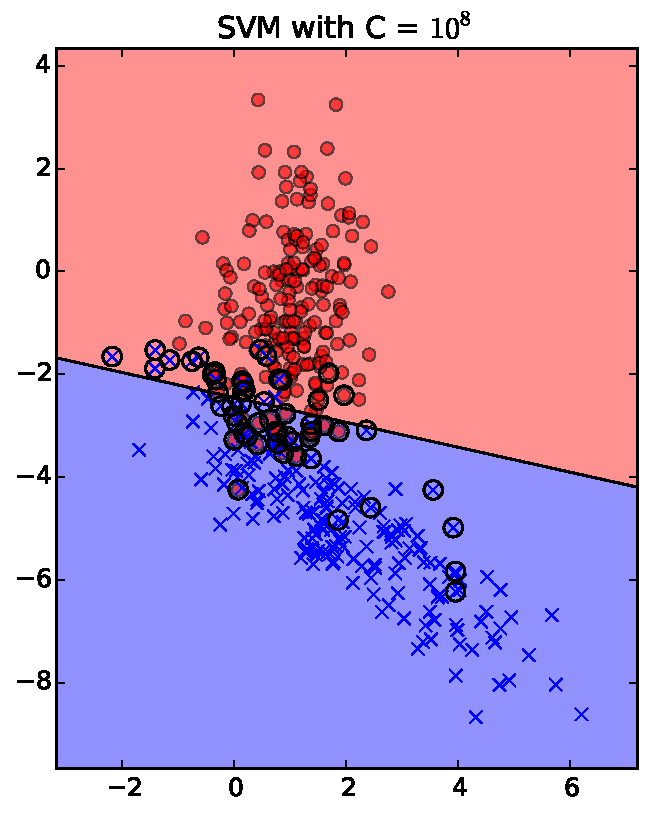
\includegraphics[width=0.2\textwidth]{SVM_C_8.pdf}
\end{center}
\end{frame}

\begin{frame}[fragile,allowframebreaks=0.8]
 {Kernel Trick}
\begin{columns}[onlytextwidth]
\column{0.79\textwidth}
\begin{itemize}
\item The SVM can be extended to nonlinear boundaries using the \textit{kernel trick}.
\item The kernel trick essentially maps the data into a higher dimension and designs the linear SVM there.
\item For example, the top plot can be generated as follows:
\begin{itemize}
\item Map the 2D samples into 3D: $(x,y) \mapsto (x^2, y^2, \sqrt{2}x y)$
\item Train the SVM with the new 3D samples.
\item The decision boundary is linear in 3D but nonlinear in 2D.
\end{itemize}
\item However, this explicit transformation is slow; the kernel trick does the same thing
implicitly.
\end{itemize}
\column{0.21\textwidth}
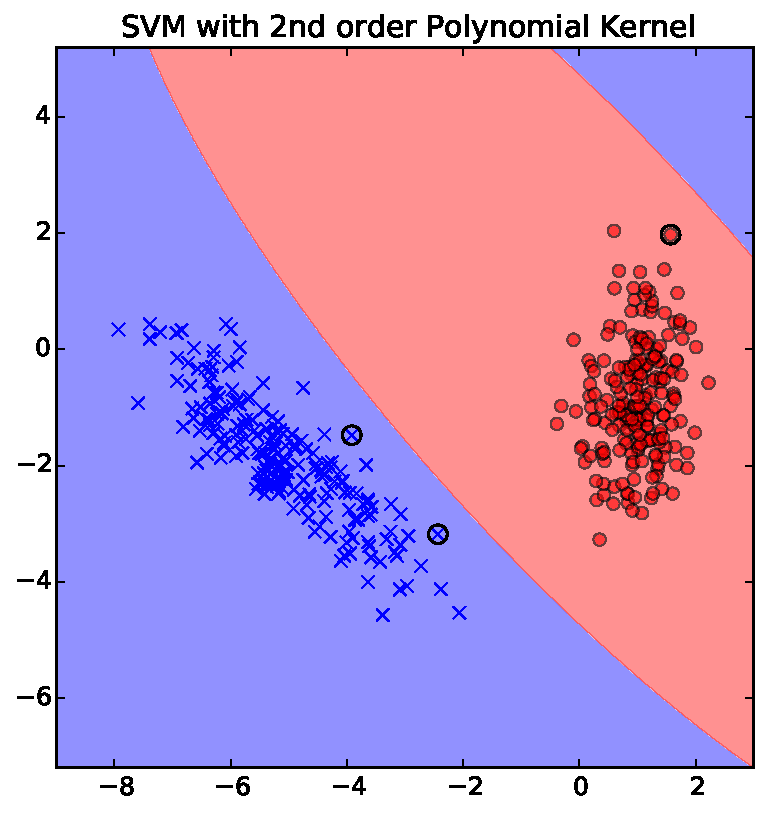
\includegraphics[width=\columnwidth]{SVM_boundary_poly2.pdf}\\
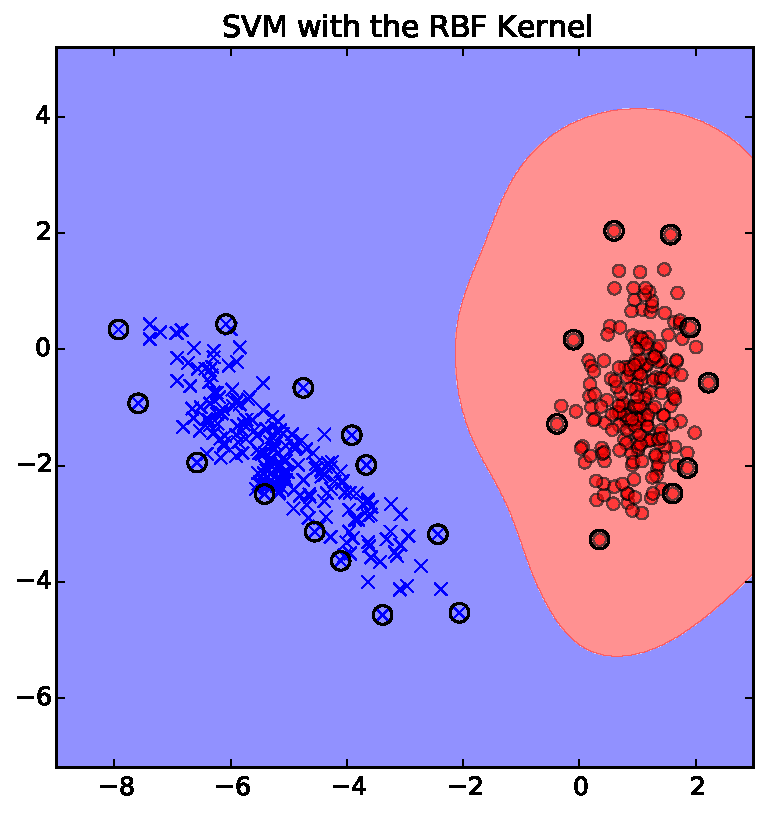
\includegraphics[width=\columnwidth]{SVM_boundary_RBF.pdf}
\end{columns}
\end{frame}

\begin{frame}[fragile,allowframebreaks=0.8]
 {Kernel Trick}
\begin{columns}[onlytextwidth]
\column{0.79\textwidth}
\begin{itemize}
\item It can be shown that substitution of the dot product by some nonlinear
function is equivalent to the explicit mapping.
\item More specifically, an algorithm can be kernelized by inserting
a kernel function $\kappa(\x,\y)$ in place of all dot products
$\x \cdot \y$.
\item It can be shown that under certain conditions on the kernel (\textit{e.g.}, positive semidefiniteness),
this is equivalent to an explicit mapping.
\item A lot of research has been done on the relation of kernel and the corresponding mapping.
\item However, we take a more practical approach and only consider an example.
\end{itemize}
\column{0.21\textwidth}
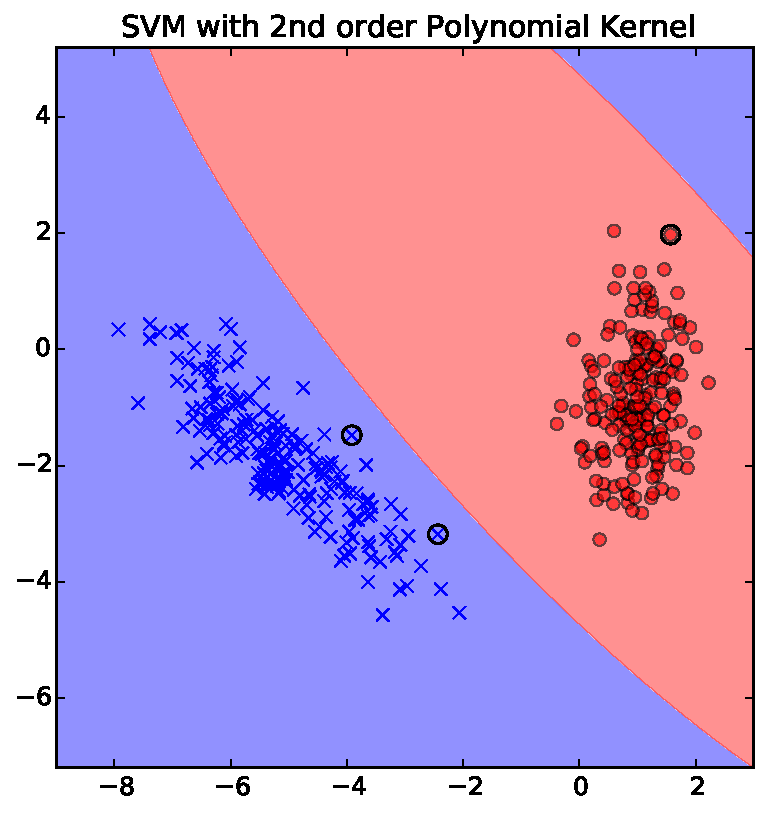
\includegraphics[width=\columnwidth]{SVM_boundary_poly2.pdf}\\
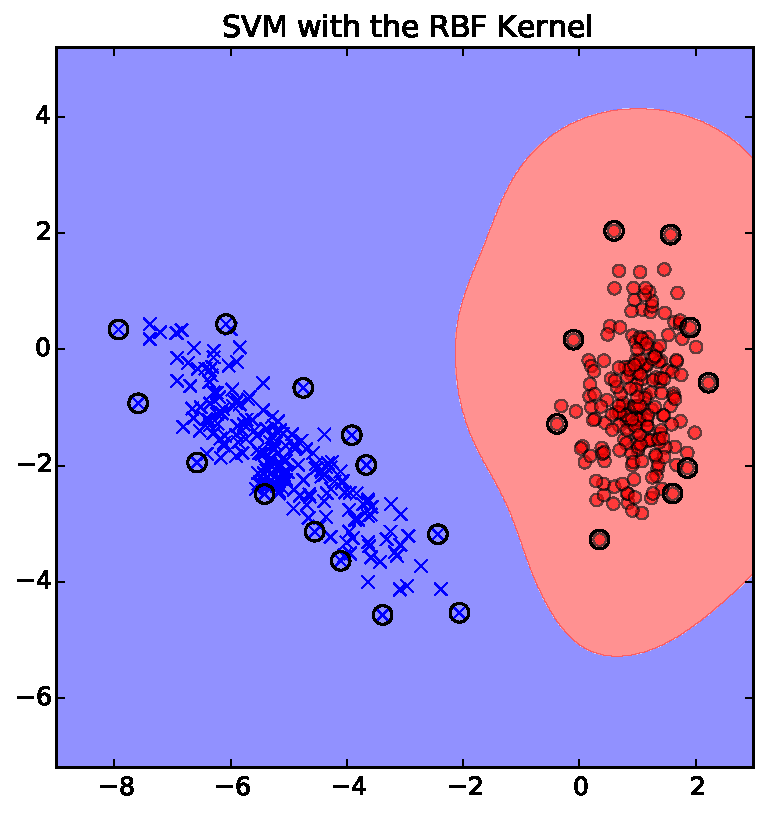
\includegraphics[width=\columnwidth]{SVM_boundary_RBF.pdf}
\end{columns}
\end{frame}

\begin{frame}[fragile,allowframebreaks=0.8]
 {Kernel Trick}
\begin{itemize}
\item As an example, consider what happens when the inner product of 2D vectors $\x = (x_1,x_2)$ and $\y = (y_1, y_2)$ is substituted by
its second power:
\[
\kappa(\x, \y) = \left(\x \cdot \y \right)^2
\]
\item We can expand the kernel as follows
\begin{align*}
\kappa(\x, \y) &= \left(\x \cdot \y \right)^2\\
&= \left(x_1y_1 + x_2y_2\right)^2\\
&= (x_1y_1)^2 + (x_2y_2)^2 + 2x_1y_1x_2y_2
\end{align*}
\item The result can be cleverly rearranged to make it look like a dot product in 3D:
\begin{align*}
\kappa(\x, \y) &= (x_1y_1)^2 + (x_2y_2)^2 + 2x_1y_1x_2y_2\\
&= (x_1y_1)^2 + (x_2y_2)^2 + (\sqrt{2}x_1x_2)(\sqrt{2}y_1y_2)\\
&= \left(x_1^2, x_2^2, \sqrt{2}x_1x_2\right) \cdot \left(y_1^2, y_2^2, \sqrt{2}y_1y_2\right)
\end{align*}
\eject
\item Thus, the following two things are equivalent:
\begin{itemize}
\item \textbf{Explicit Mapping}: Transform 2D data into 3D explicitly and fit the SVM with transformed data:
\[
\begin{pmatrix}
u \\ v
\end{pmatrix}
\mapsto 
\begin{pmatrix}
u^2\\
v^2\\
\sqrt{2}u v
\end{pmatrix}
\]
\item \textbf{Implicit Mapping}: Substitute each dot product in the SVM algorithm by the
kernel $\kappa(\x, \y) = \left(\x \cdot \y \right)^2$ and fit with original 2D data.
\end{itemize}
\end{itemize}
\end{frame}


\begin{frame}[fragile,allowframebreaks=0.8]
 {Popular Kernels}
\begin{itemize}
\item As mentioned, there is lot of literature on kernels. Popular ones include
\begin{itemize}
\item \textbf{Linear Kernel:} $\kappa(\x, \y) = \x \cdot \y$. This is the basic SVM with no mapping.
\item \textbf{Polynomial Kernel:} $\kappa(\x, \y) = (\x \cdot \y)^d$. Raises dot product to $d$'th power.
\item \textbf{Inhomogeneous Polynomial Kernel:} $\kappa(\x, \y) = (\x \cdot \y + 1)^d$. Similar to polynomial kernel, but produces a bit more dimensions.
\item \textbf{Sigmoid Kernel:} $\kappa(\x, \y) = \mathop{\text{tanh}}(a\x\cdot \y + b)$, with $a>0$ and $b < 0$.
\item \textbf{Gaussian Kernel:} $\kappa(\x, \y) = \exp\left(-\frac{\|\x - \y\|^2}{2\sigma^2} \right)$. Probably the most widely used kernel.
Also known as \textbf{Radial Basis Function (RBF)} kernel.
\end{itemize}
\item The RBF kernel is special in the sense that it corresponds to a mapping into an
\textbf{infinite dimensional} vector space.
\item In addition to the mathematical excitement, the RBF kernel is often the best performing one, as well.
\end{itemize}
\end{frame}

\begin{frame}[fragile,allowframebreaks=0.8]
{SVM in Scikit-Learn}
\begin{columns}[onlytextwidth]
\column{0.55\textwidth}
\begin{lstlisting}
# Training code:
from sklearn.svm import SVC
# Alternatively: from sklearn.svm import LinearSVC

# Kernels include: "linear", "rbf", "poly", "sigmoid"
# C is the penalty term (default = 1)
clf = SVC(kernel = 'linear', C = 1)

# X contains all samples, and y their class
# labels: y = [0,1,1,0,...]
clf.fit(X, y)
\end{lstlisting}
\begin{lstlisting}
# Testing code:
>>> clf.coef_ # This is our w vector (linear case)
array([[ 0.72817808,  0.26866005]])  

>>> clf.intercept_ # This is the threshold
array([ 3.31965658])

>>> clf.predict([[-4,-2], [-2,0]])
array([ 0.,  1.])

>>> clf.support_vectors_
array([[-2.43263229, -3.18119051],
       [ 0.34905559, -3.27417889],
       [-0.38544996, -1.28336992]])
\end{lstlisting}
\column{0.5\textwidth}
\begin{itemize}
\item Scikit-Learn wraps the LibSVM and LibLinear libraries (latter is linear kernel optimized).
\end{itemize}
\centerline{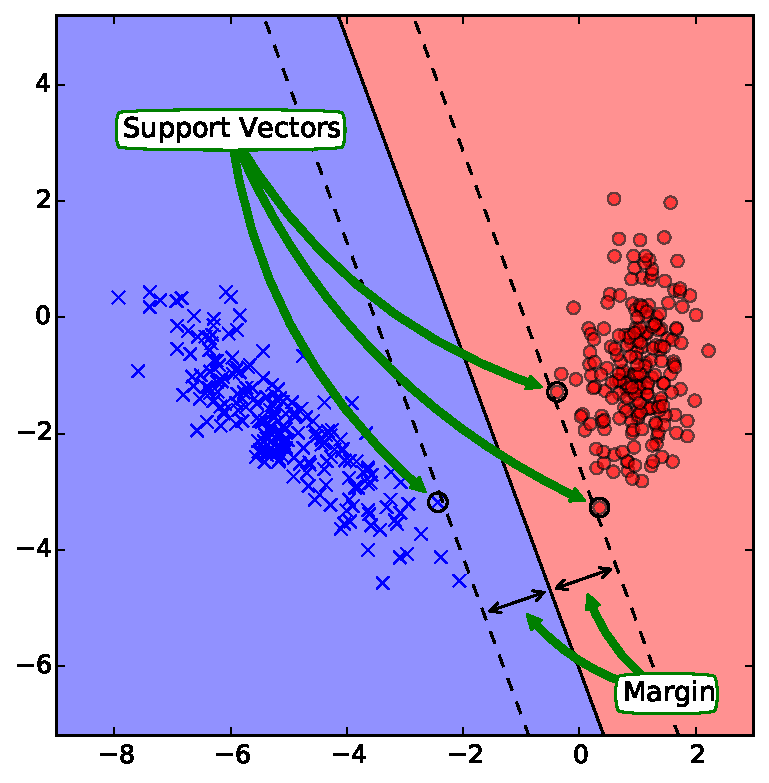
\includegraphics[width=0.8\columnwidth]{SVM_boundary.pdf}}
\end{columns}
\end{frame}

\begin{frame}[fragile,allowframebreaks=0.8]
{Multiclass SVM}
\begin{itemize}
\item SVM is inherently two-class.
\item Generalization to many classes is done by comparing pairs of classes.
\item For each class, we train a SVM that classifies this class vs. all others.
\item Scikit-Learn provides a few \textit{meta-classifiers} for this purpose.
\begin{itemize}
\item \verb+multiclass.OneVsRestClassifier+ compares each class vs. all others (requires $K$ classifiers)
\item \verb+multiclass.OneVsOneClassifier+ compares all class pairs (requires $K(K-1) / 2$ classifiers)
\end{itemize}
\eject
\item A further extension is \emph{multilabel} classification, where several classes can be
present simultaneously.
\item Targets are presented as binary indicators: 
\begin{lstlisting}
>>> from sklearn.preprocessing import MultiLabelBinarizer
>>> y = [[2, 3, 4], [2], [0, 1, 3], [0, 1, 2, 3, 4], [0, 1, 2]]
>>> MultiLabelBinarizer().fit_transform(y)
array([[0, 0, 1, 1, 1], # Classes 2,3,4 are "on"
       [0, 0, 1, 0, 0], # Class 3 is "on"
       [1, 1, 0, 1, 0], # ...
       [1, 1, 1, 1, 1],
       [1, 1, 1, 0, 0]])
\end{lstlisting}
\end{itemize}
\begin{columns}
\column{0.8\textwidth}
\begin{itemize}
\item Occurs often in, \emph{e.g.,} image recognition problems: "What is shown in this picture."
\item For example, the following attributes are "on" in the attached picture:
\{"\textbf{fly}", "\textbf{flower}", "\textbf{summer}"\}
\end{itemize}
\column{0.2\textwidth}
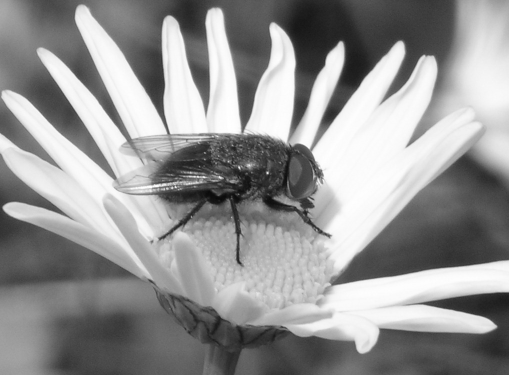
\includegraphics[width=\columnwidth]{karpanen.png}
\end{columns}
\end{frame}

\begin{frame}[fragile,allowframebreaks=0.8]
{Multiclass SVM}
\begin{columns}[onlytextwidth]
\column{0.5\textwidth}
\begin{lstlisting}
# Training code:
from sklearn.svm import LinearSVC
from sklearn.multiclass import OneVsRestClassifier
from sklearn.multiclass import OneVsOneClassifier

clf_ova = OneVsRestClassifier(LinearSVC())
clf_ova.fit(X, y)

clf_ovo = OneVsOneClassifier(LinearSVC())
clf_ovo.fit(X, y)
\end{lstlisting}
\begin{lstlisting}
# Testing code:
>>> clf_ova.predict(np.array([[2,-3.2], [4,-2]]))
array([ 2.,  3.])

>>> clf_ovo.predict(np.array([[2,-3.2], [4,-2]]))
array([ 1.,  3.])

>>> len(clf_ova.estimators_)
3
\end{lstlisting}
\column{0.5\textwidth}
\begin{itemize}
	\item \verb+SVC()+ in fact implements OvO heuristic inherently.
	\item \verb+LinearSVC()+ does not, so let's use that as our example.
\end{itemize}
\begin{center}
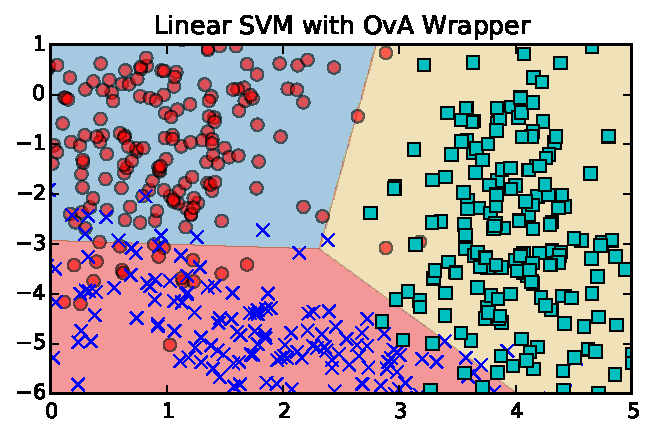
\includegraphics[width=0.6\columnwidth]{3Class_SVM_classes_OvA.pdf}\\
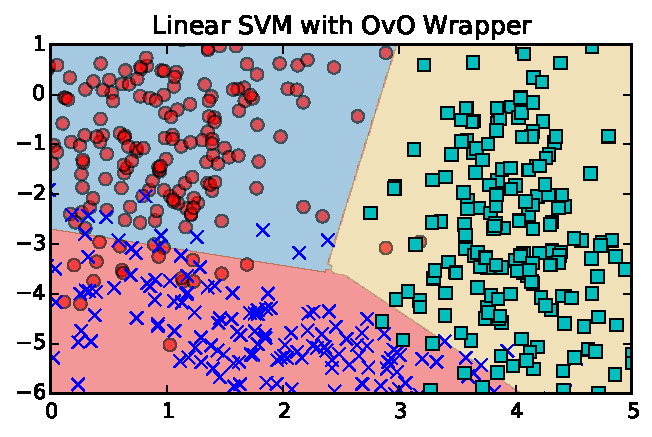
\includegraphics[width=0.6\columnwidth]{3Class_SVM_classes_OvO.pdf}
\end{center}
\end{columns}
\end{frame}


\begin{frame}{Logistic Regression}
\begin{itemize}
\item The third member of linear classifier family is \textit{Logistic Regression} (LR).
\item Unlike the other two, LR is \textit{probabilistic}, \textit{i.e.}, it models the 
class probabilities instead of plain class memberships.
\item For two-class case ($c\in\{0,1\}$), the model is:
\[
p(c=1 \mid \x) = \frac{1}{1 + \exp[-(\w^T\x + b)]}.
\]
\end{itemize}
\begin{columns}[onlytextwidth]
\column{0.7\textwidth}
\begin{itemize}
\item Also: $p(c=0\mid\x) =  1-p(c=1\mid\x)$.
	\item In essence, the model maps the projection $\w^T\x + b$
	through the sigmoid function (thus limiting the range to $[0,1]$).
\end{itemize}
\column{0.35\textwidth}
\centerline{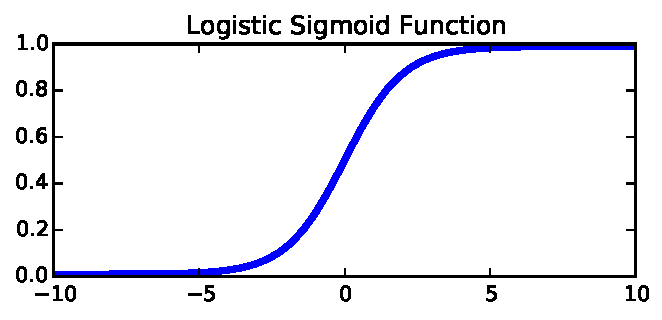
\includegraphics[width=\textwidth]{sigmoid.pdf}}
\end{columns}
\end{frame}


\begin{frame}{Logistic Regression}
\begin{columns}[onlytextwidth]
\column{0.7\textwidth}
\begin{itemize}
\item The model is illustrated in the flowgraph:
\begin{itemize}
	\item The samples are projected to 1D using the learned weights $\w$ and $b$.
	\item The resulting "class scores" are mapped through the logistic function,
	which transforms the scores to probabilities $p(c = 1 \mid \x)\in[0,1]$.
\end{itemize}
\end{itemize}
\begin{columns}[onlytextwidth]
\column{0.79\textwidth}
\begin{itemize}
	\item The probability estimates can also be mapped back to 2D,
	as shown in the figure on the right.
\end{itemize}
\vspace*{2cm}
\column{0.35\textwidth}
	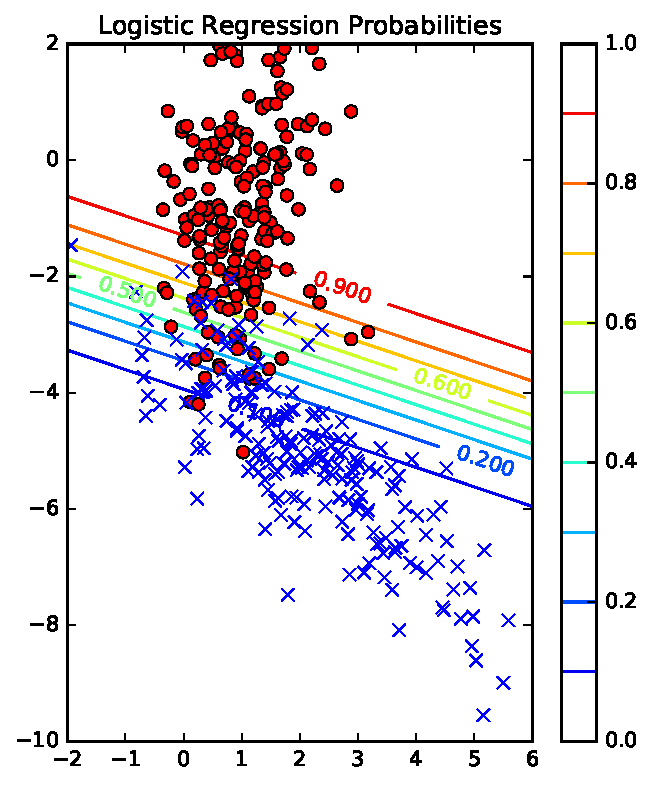
\includegraphics[width=\textwidth]{LR_prob_2D.pdf}
\end{columns}
\column{0.21\textwidth}
\begin{center}
	\vspace*{-1cm}
	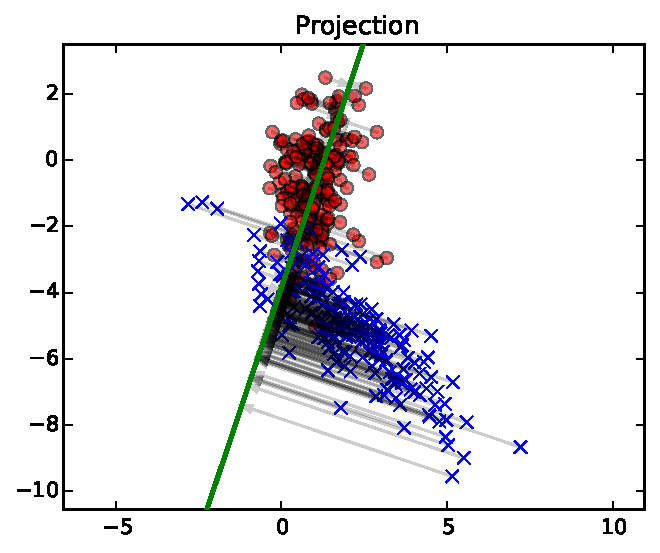
\includegraphics[width=\textwidth]{LR_proj.pdf}\\
	\vspace*{-0.2cm}$\downarrow$\\
	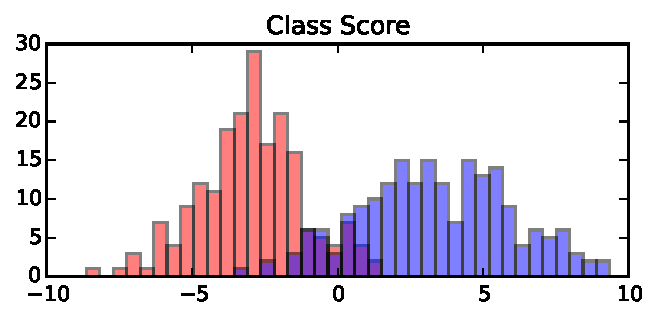
\includegraphics[width=\textwidth]{LR_score.pdf}\\
	\vspace*{-0.2cm}$\downarrow$\\
	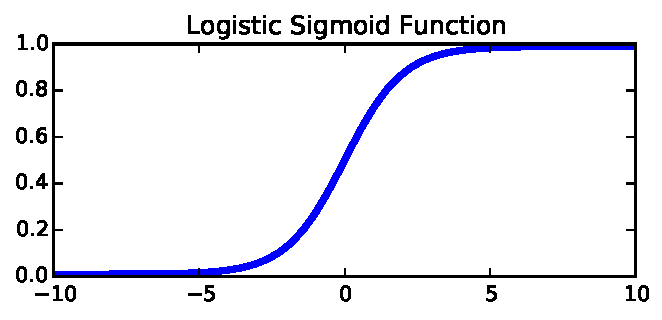
\includegraphics[width=\textwidth]{sigmoid.pdf}\\
	\vspace*{-0.2cm}$\downarrow$\\
	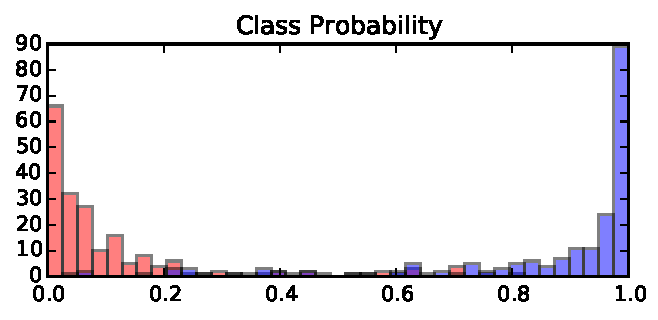
\includegraphics[width=\textwidth]{LR_prob.pdf}
\end{center}
\end{columns}
\end{frame}

\begin{frame}{Training Logistic Regression Models}
\begin{itemize}
\item Logistic regression is trained by \emph{maximum likelihood}.
\item In other words, we maximize the likelihood of observing these
data points with respect to model parameters.
\item The likelihood of samples $\X = [\x_0, \x_1, \ldots, \x_{N-1}]$ with class labels
$y_0, y_1,\ldots, y_{N-1} \in \{1,2,\ldots, K\}$ to have occurred from
the model with parameters $\thb$ is
\[
p(\X \mid \thb) = \prod_{n = 0}^{N-1} p_{y_n}(\x_n; \thb).
\]
\item As usual, we consider the log-likelihood instead:
\[
\ln p(\X \mid \thb) = \sum_{n = 0}^{N-1} \ln p_{y_n}(\x_n; \thb).
\]
\end{itemize}
\end{frame}

\begin{frame}[allowframebreaks]{Training Logistic Regression Models}
\begin{itemize}
\item Due to simplicity, we will continue with the two-class case only.
\item Let's label the classes as $y_k\in\{-1,1\}$, because this will simplify the notation later.
\item Also: let's hide the constant term $b$ by catenating it at the end of $\w$:
\[
\w \leftarrow [\w, b]\quad\text{and}\quad \x \leftarrow [\x, 1]
\]
\item The likelihood for classes $-1$ and $1$ are now
\begin{align*}
p(\x_n \mid y_n = 1) &= \frac{1}{1 + \exp(-\w^T\x_n)}\\
p(\x_n \mid y_n = -1) &= 1-\frac{1}{1 + \exp(-\w^T\x_n)}\\
&= \frac{(1 + \exp(-\w^T\x_n)) - 1}{1 + \exp(-\w^T\x_n)}\\
&= \frac{\exp(-\w^T\x_n)}{1 + \exp(-\w^T\x_n)}\\
&= \frac{1}{\exp(\w^T\x_n) + 1}
= \frac{1}{1 + \exp(\w^T\x_n)}
\end{align*}
\end{itemize}
\end{frame}

\begin{frame}[allowframebreaks]{Training Logistic Regression Models}
\begin{itemize}
\item Now $p(\x_n \mid y_n = 1)$ and $p(\x_n \mid y_n = -1)$ are almost the same form
and can be conveniently combined into one formula:
\[
p(\x_n \mid y_n) = \frac{1}{1 + \exp(-y_n\w^T\x_n)}
\]
\item The likelihood for all samples $\X = [\x_0, \x_1, \ldots, \x_{N-1}]$ is now
\[
p(\X \mid \w, \y) = \prod_{n = 0}^{N-1} \frac{1}{1 + \exp(-y_n\w^T\x_n)}
\]
\item The log-likelihood becomes
\begin{align*}
\ln p(\X \mid \w, \y) &= \sum_{n = 0}^{N-1} \ln 1 - \ln(1 + \exp(-y_n\w^T\x_n))\\
&= -\sum_{n = 0}^{N-1} \ln(1 + \exp(-y_n\w^T\x_n)).
\end{align*}
\end{itemize}
\end{frame}

\begin{frame}[allowframebreaks]{Training Logistic Regression Models}
\begin{itemize}
\item In order to maximize the likelihood, we can equivalently minimize the 
\emph{logistic loss function}:
\[
\text{log-loss} = \sum_{n = 0}^{N-1} \ln(1 + \exp(-y_n\w^T\x_n)).
\]
\item There exists several algorithms for minimization of logistic loss, \emph{e.g.,}
\begin{itemize}
	\item Iterative Reweighted Least Squares \textbf{(IRLS)} is an algorithm specifically tailored for this kind of problems. Used by \texttt{statsmodels.api.Logit} and \texttt{statsmodels.api.MNLogit}.
	\item Optimization theory based approaches. Since $\ln p(\X \mid \thb)$ is convex, in principle any optimization approach can be used. 
	\texttt{scikit-learn} uses something called \emph{Trust Region Newton Algorithm}.
\end{itemize}
\end{itemize}
\end{frame}

\begin{frame}[allowframebreaks]{Training Logistic Regression Models}
\begin{itemize}
\item The optimization theory approach has become dominant, for two reasons:
\begin{enumerate}
	\item The SVM training can also be posed in the same framework: minimize the \emph{hinge loss}:
	\[
	\text{hinge-loss} = \max(0, 1-y_n\w^T\x_n).
	\]
	\item A general purpose optimizer can minimize modified losses, as well. Most importantly,
	one can add a penalty term into the loss function; \emph{e.g.,}
	\[
	\text{penalized log-loss} = \sum_{n = 0}^{N-1} \ln(1 + \exp(-y_n\w^T\x_n)) + C \w^T\w
	\]
	where the latter term favors small coefficients in $\w$. We will return to this
	technique called \emph{regularization} later.
\end{enumerate}
\end{itemize}
\end{frame}

\begin{frame}[fragile]{Example: Effect of Regularization Parameter $C$}
\begin{columns}
\column{0.53\textwidth}
\begin{lstlisting}
from sklearn.cross_validation import train_test_split

# Split data to training and testing
X_train, X_test, y_train, y_test = \
      train_test_split(X, y, test_size = 0.2)

# Test C values -4, -3, ..., 2
C_range = 10.0 ** np.arange(-4, 3)
clf = LogisticRegression()

for C in C_range:

   clf.C = C
   clf.fit(X_train, y_train)
   y_hat = clf.predict(X_test)
   accuracy = 100.0 * np.mean(y_hat == y_test)

   print ("Accuracy for C = %.2e is %.1f %% (||w|| = %.4f)" % \
         (C, accuracy, np.linalg.norm(clf.coef_)))
\end{lstlisting}
\begin{lstlisting}
# Code output for the 3-class example data:

Accuracy for C = 1.00e-04 is 50.8 % (||w|| = 0.0660)
Accuracy for C = 1.00e-03 is 59.2 % (||w|| = 0.3332)
Accuracy for C = 1.00e-02 is 73.3 % (||w|| = 1.0372)
Accuracy for C = 1.00e-01 is 88.3 % (||w|| = 2.0715)
Accuracy for C = 1.00e+00 is 90.8 % (||w|| = 3.2153)
Accuracy for C = 1.00e+01 is 91.7 % (||w|| = 3.7732)
Accuracy for C = 1.00e+02 is 91.7 % (||w|| = 3.8704)
\end{lstlisting}
\column{0.4\textwidth}
\begin{itemize}
	\item In this example, we train the LR classifier with a range of values for parameter C.
	\item Each C value can be set inside a for loop as \mbox{\texttt{clf.C = <new value>}}
	\item We test the accuracy on a separate test data extracted from the complete data set.
\end{itemize}
\end{columns}
\end{frame}


\begin{frame}{Multiclass Logistic Regression}
There are two ways to extend LR to multiclass.
\begin{itemize}
\item[\ding{202}] A straightforward way would just normalize the exponential terms to sum up to 1:
\begin{align*}
p(c = k\mid \x) = \frac{\exp(\w_k^T\x + b_k)}{\sum_{j=1}^K\exp(\w_j^T\x + b_j)}
\end{align*}
However, one of the terms is unnecessary, because the probabilities add up to 1.
\item[\ding{203}] Thus, we get an alternative model with fewer parameters:
\begin{align*}
p(c = k\mid \x) &= \frac{\exp(\w_k^T\x + b_k)}{1 + \sum_{j=1}^{K-1}\exp(\w_j^T\x + b_j)}, \quad k = 1,2,\ldots, K-1\\
p(c = K\mid \x) &= \frac{1}{1 + \sum_{j=1}^{K-1}\exp(\w_j^T\x + b_j)}.
\end{align*}
\end{itemize}
\end{frame}

\begin{frame}[fragile]{Multiclass Version \ding{202}}
\begin{columns}[onlytextwidth]
\column{0.83\textwidth}
\begin{itemize}
\item The first approach designs one probability model $p(c = k\mid \x)$ for each class.
\item However, the model is ill-posed: there are infinitely many solutions (by scaling).
\item Thus, the model needs to be regularized to create a unique solution.
\item This is the model given by \texttt{scikit-learn}.
\end{itemize}
\begin{lstlisting}
# Training code:
from sklearn.linear_model import LogisticRegression

clf = LogisticRegression()
clf.fit(X, y)
\end{lstlisting}
\vspace*{-0.3cm}
\begin{columns}[onlytextwidth]
\column{0.47\textwidth}
\begin{lstlisting}
# Test code:
>>> clf.predict([[1,-1], [4, -6]])
array([ 1.,  2.])

clf.predict_proba([[1,-1], [4, -6]])
array([[0.927, 0.038, 0.035],
       [0.001, 0.501, 0.498]]
\end{lstlisting}
\column{0.47\textwidth}
\begin{lstlisting}
# Model parameters:
>>> clf.coef_
array([[-1.23804226,  0.98973963],
       [-1.37272021, -1.53820378],
       [ 2.13288304,  0.54858162]])
>>> clf.intercept_
array([ 3.79924145, -3.50411623, -5.02047854])			
\end{lstlisting}
\end{columns}
\column{0.17\textwidth}
\vspace*{-1cm}
\begin{center}
	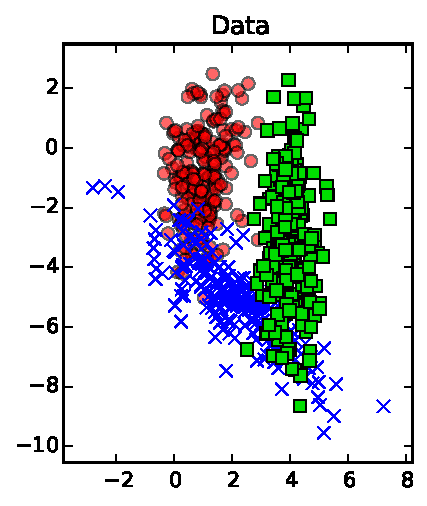
\includegraphics[width=\textwidth]{LR_3classes_data.pdf}\\
	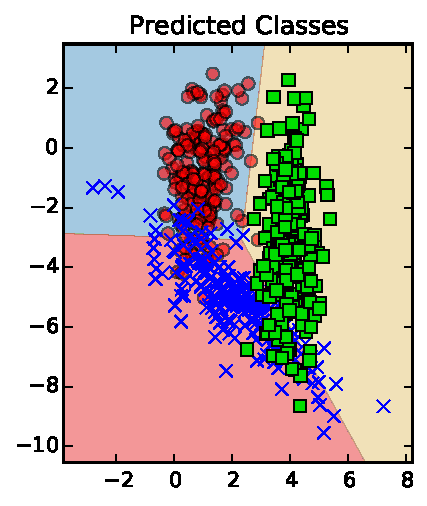
\includegraphics[width=\textwidth]{LR_3classes.pdf}\\
	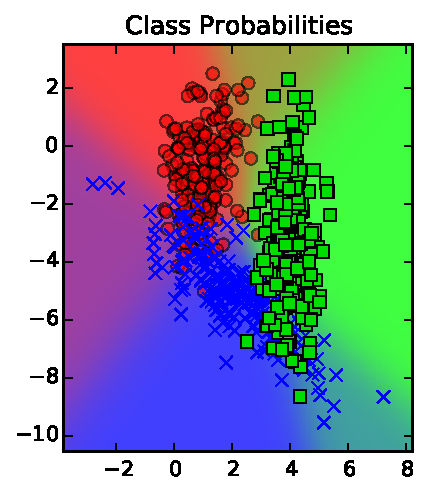
\includegraphics[width=\textwidth]{LR_3classes_prob.pdf}\\
\end{center}
\end{columns}
\end{frame}

\begin{frame}[fragile]{Multiclass Version \ding{203}}
\begin{columns}[onlytextwidth]
\column{0.83\textwidth}
\begin{itemize}
	\item The second version is historically older.
	\item Has a unique solution even without regularization.
	\item Is not implemented in \texttt{scikit-learn}, but can be found in \texttt{statsmodels} library.
\end{itemize}
\begin{lstlisting}
# Training code:
from statsmodels.api import MNLogit

# statsmodel has a bit different API.
# In reality, X should zero-mean, but
# let's simplify the code a bit here.
clf = MNLogit(y, X)
clf = clf.fit()
\end{lstlisting}
\vspace*{-0.3cm}
\begin{columns}[onlytextwidth]
\column{0.53\textwidth}
\begin{lstlisting}
# Test code:
>>> clf.predict([[1,-1], [4, -6]])
array([[0.972, 0.019, 0.009],
       [0.001, 0.471, 0.528]],

# clf.predict() gives probabilities.
# To get classes, we find the max:
>>>  clf.predict([[1,-1], [4, -6]]).argmax(axis = 1)
array([0, 2])
\end{lstlisting}
\column{0.44\textwidth}
\begin{lstlisting}
# Model parameters:

>> clf.params
array([[-0.06122776,  2.82418605],
       [-2.00590479, -0.4564178 ]])

# Note: only two sets of weights.
# Note2: no intercept; assumes zero mean
\end{lstlisting}
\end{columns}
\column{0.17\textwidth}
\vspace*{-1cm}
\begin{center}
	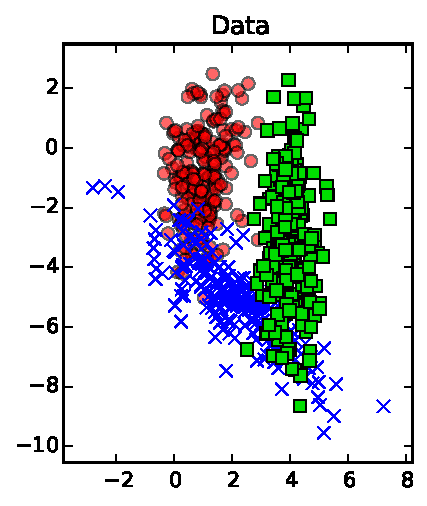
\includegraphics[width=\textwidth]{LR_3classes_data.pdf}\\
	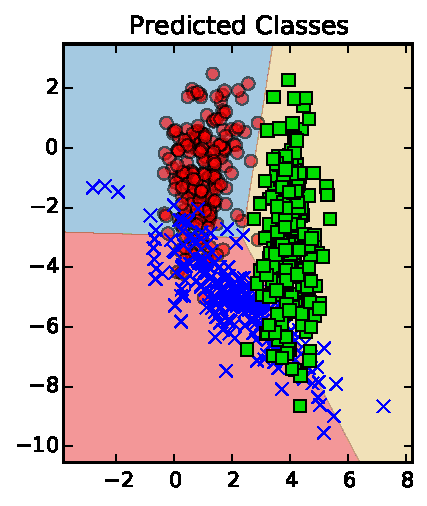
\includegraphics[width=\textwidth]{LR_3classes_stf.pdf}\\
	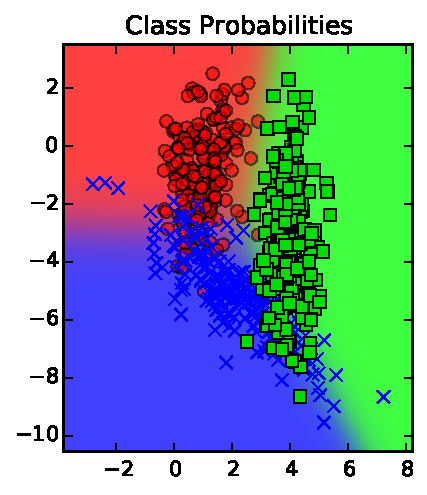
\includegraphics[width=\textwidth]{LR_3classes_prob_stf.pdf}\\
\end{center}
\end{columns}
\end{frame}

\end{document}

